\documentclass[draft]{agujournal2019}
\usepackage{amsmath}
\usepackage{url} 
\usepackage{lineno}
\usepackage[inline]{trackchanges} % track changes. 
\usepackage{soul}
\linenumbers

\draftfalse

\journalname{JGR: Earth Surface}

\begin{document}

\title{Linking landslide patterns to transient landscapes in the northern Colombian Andes}

\authors{Edier Aristizábal\affil{1,2}, Oliver Korup\affil{2,3}}

\affiliation{1}{Departamento de Geociencias y Medio Ambiente, Universidad Nacional de Colombia, Medellín, Colombia}
\affiliation{2}{Institute of Environmental Science and Geography, University of Potsdam, Germany}
\affiliation{3}{Institute of Geosciences, University of Potsdam, Germany}

\correspondingauthor{Oliver Korup}{korup@uni-potsdam.de}

\begin{keypoints}
\item We explore potential links between drainage network dynamics and landslide patterns in the tectonically active Colombian Andes.
\item The distribution of $\sim$14,000 landslides shows little spatial coincidence with varying channel steepness, but older landslides tend to be closer to actively migrating divides.
\item Clustering of catchment hypsometry instead objectively identifies four progressive stages of catchment transience with differing landslide densities.
\end{keypoints}

\begin{abstract}
Landslides are among the most recognizable evidence of hillslope erosion in tectonically active mountains. Yet, how much of the distribution of landslides of different ages relates to, or is inherited from, the pattern of topographic metrics of landscape evolution remains partially unresolved, and especially so in tropical areas. We derive such metrics for 650 catchments of 10$^1$-10$^2$ km$^2$ in size, including their mean hypsometric integral, local relief, geological lineament density, and steepness variations and knickpoint density of river channels as proxies of tectonic activity. We test how these proxies match with, if not explain, the distribution of some 14,000 prehistoric and modern landslides in the northern Colombian Andes. A $K$-means cluster analysis of catchment hypsometry reveals four distinct groups of catchments. We interpret these groups to reflect different states of transience with clear contrasts in mean local relief, average hillslope inclination, channel steepness, and landslide density. We propose that tectonic uplift, base-level changes, and passing waves of incision control these different states of transience. Yet, we find that landslides occur widely without much spatial association to, or amassing near, major channel knickpoints. This observation reflects what we would expect from a threshold landscape in which landslides abound irrespective of contrasts in local river incision rates. Still, we notice a pronounced amassing of landslides near transient divides, where prehistoric landslides are preferentially preserved. In summary, we infer that, in our study area at least, differences in catchment hypsometry might be more useful to track potential tectonic controls on landslide patterns than comparing these to knickpoint distributions or channel metrics.
\end{abstract}

\subsection*{Plain language summary}
Landslides are common signs of hillslope erosion in tectonically active mountains. Yet, it is not fully clear how much the distribution of landslides is influenced by topographic features that mark stages of landscape evolution, particularly in tropical areas. We analyzed 650 catchments in the Colombian Andes in terms or their local relief, geological features, and river steepness as measures of tectonic activity. We used a clustering analysis to identify four distinct groups of catchments, which broadly reflect different stages of landscape change, and especially river downcutting, due to these tectonic forces. However, we also found that landslides do not consistently occur near river channels where major erosion happens, Instead, landslides are sprawled more widely across the landscape. Still, prehistoric landslides tend to be preserved nearer than recent landslides to catchment boundaries that actively shift because of river erosion. Our results suggest that information about catchment elevation may be useful for understanding the tectonic influence on landslide patterns.

%%%%%%%%%%%%%%%%%%%%%%%%%%%%%%%%%%%%%%%%%%%%%%%%%%%%%%
\section{Introduction}
\par Modern views of landscape evolution emphasize the dynamic interaction between tectonic activity and climatically modulated shifts of mass across the land surface \cite{Davies2021, Whittaker2012, Irasema2002}. Tectonic or climate perturbations may cause transient states, but landscapes move toward a dynamic equilibrium in which rock uplift and denudation are balanced on average \cite{Whittaker2012, Wobus2006, Whipple2004}. River networks are primary conveyors by which perturbations propagate through the landscape, and force adjacent hillslopes to respond to changes in base level \cite{Whipple2004, howard1994}. The geometric configuration of rivers and hillslopes thus encodes valuable information on tectonic and climatic disturbances \cite{whipple2017, stock1999}, offering insights into the dominant geomorphic processes, which in mountains often involve abundant landsliding \cite{Larsen2012, korup2010, Montgomery2002, Campforts2020, Broeckx2020}. 

\par Several authors emphasize how landslides might control landscape response to catchment perturbations \cite{montgomery2001slope}. Numerical landscape evolution models built on stream-power models incorporate hillslope-channel coupling and landsliding via mechanistic threshold criteria. For example, \citeA{Egholm2013} simulated a reciprocal relationship between channel incision and landslides. Their model showed positive feedback when landslides increased sediment input and accelerated fluvial incision, whereas a negative feedback emerged where excess sediment protected the river bed from erosion. \citeA{roering2015} showed how changes in rock uplift and incision alter the frequency and pattern of active landslides in the northern California Coast Ranges. The authors proposed that areas with greater uplift rates have larger, faster, and more frequent landslides. A landscape evolution model by \citeA{Campforts2020, Campforts2022} featured stochastic landsliding and its effect on fluvial sediment dynamics and showed that, as rock-uplift rates increased, so did the frequency and magnitude of landslides, whereas drainage density and stream concavity decreased.

\par Despite these and similar studies, the spatial patterns of landsliding remain poorly understood beyond the scope of individual triggers such as earthquakes or rainstorms \cite{yanites2018}. While susceptibility studies attempt to explain landslide distribution in space, they concentrate on the hillslope scale and use local terrain indices, slope material properties, or land-cover attributes as statistical predictors \cite{reichenbach2018, soeters1996, montgomery1994}. Yet, how these possible controls play out in terms of entire landslide patterns instead of local, pixel-wise, susceptibility remains uncertain, and thus often described as stochastic \cite{Benda1997}. 

\par A broader view is that landslides form as a local hillslope response to upstream knickpoint migration in response to base-level fall into catchments in disequilibrium \cite{Wobus2006, hovius2006, Whipple2002}. Thus, the dynamics of the channel network should eventually control landslide distribution \cite{montgomery1994, burbank1996}. \citeA{Larsen2012} supported this notion by reporting a significant correlation between landslide frequency, exhumation rates, and stream power in the eastern Himalayas. \citeA{tsou2017} used river and hillslope morphometry to show that transient hillslopes resulting by successive rejuvenated river incision control the distribution of deep-seated landslides and long-term slope stability in southwestern Japan. \citeA{Gallen2011} noted a similar pattern in the southern Appalachians, where local relief is higher, hillslopes steeper, and landslides more abundant in tributary catchments downstream of major knickpoints. The authors used hypsometric analyses to propose a model for determining different evolutionary stages of landscape development. This model posits that the hypsometric distribution of a catchment in equilibrium tends to be skewed toward lower elevations. When a perturbation occurs, it creates a distinct peak in the hypsometric distribution that migrates to higher elevations, moving farther away from a state of equilibrium. 

\par Most of these studies focused on tectonically active mountains in temperate climate zones. In contrast, insights are rare from tropical regions, where rainfall is distinctly seasonal, rates of chemical weathering are high, and the geomorphic legacy of glaciers is minimal. Here, we choose the northern Colombian Andes as an example of a tectonically active and tropical mountain belt dotted by numerous landslides. Landslides are a major natural hazard in Colombia \cite{gomez2023spatial, aristizabal2020}, though most studies have ignored the potential legacy of tectonic uplift and landscape evolution on where landslides occur. Hence, we examine whether the pattern of prehistoric and recent landslides is linked to metrics of landscape evolution, especially those that help to infer hillslopes and river channel dynamics. In particular, we test the model proposed by \citeA{Gallen2011}. We aim to evaluate whether digital topographic data can effectively identify stages of landscape evolution and tectonic activity, and assess their influence on the spatial distribution of observed landslides.

%%%%%%%%%%%%%%%%%%%%%%%%%%%%%%%%%%%%%%%%%%%%%%%%%%%%%%%%%%%%%
\section{Study area}
\par The Colombian Andes have unique geomorphic and hydroclimatological characteristics that result from their tectonic and equatorial setting (Fig.~\ref{fig:marco}). In the northern Andes, geological features are controlled by the diagonal convergence of the Nazca and Caribbean oceanic plates with the South American continental plate \cite{Cediel2003, acosta2007, trenkamp2002}. This transpressional accretion features two distinct crustal blocks: the Northern Andean Block (NAB) is moving in a north-westward direction, whereas the Panamá-Chocó Block (PCB) is moving in a south-eastward direction, in relation to the South American Plate \cite{kellogg1995}. The accretion of the PCB caused the Nazca Plate to rupture at about 5°N, causing flat slab subduction in the north \cite{Taboada2000}. In contrast, the south has a steeper subduction angle and active volcanoes \cite{perez2021, restrepo2019, farris2011, Taboada2000, mann1990} (Fig.~\ref{fig:marco}). 

\par Our study area is located in the Colombian Andes north of 5°N, and covers the Western Cordillera (WC) and high-elevation ($\sim$2500 m a.s.l.), low-relief, and flat-topped erosional surfaces of the Central Cordillera (CC), known as the Antioqueño Plateau (AP) that is deeply incised by the Nechí River, the main tributary of the Cauca River. The study area features the Cauca canyon (Fig.~\ref{fig:geologia}A), and is bounded by broad alluvial flats to the west of the Atrató River, to the east by the Magdalena River, and to the north by the Cauca River.

\par The study area covers some 48,000~km$^2$, which we divided into 650 catchments of similar areas and stream orders. About 75\% of these catchments drain less than 100~km$^{2}$ each, with a median area of 36~km$^{2}$. The catchments have average slopes between 15° and 25° with a relief ranging from 180~m to 380~m, and up to 750~m in the northern Cauca canyon (Fig.~\ref{fig:rainfall}). Narrow valleys bounded by steep slopes characterize the WC and eastern flanks of the CC. 

\par The study area has a diverse geological framework comprising volcanic, intrusive, oceanic, metamorphic, sedimentary, ultramafic rocks, and unconsolidated sedimentary deposits (Figure \ref{fig:geologia}A). The volcanic units, primarily andesitic to basaltic in composition, are interbedded with volcaniclastic deposits, reflecting active volcanic processes during Cretaceous to Paleogene times. Intrusive rocks include granitic and dioritic bodies emplaced during the Late Cretaceous and early Tertiary, indicative of magmatic arc activity associated with subduction zones \cite{restrepo2019}. Oceanic rocks, such as basalts and pelagic cherts, represent remnants of ancient oceanic crust and associated marine sediments \cite{Cediel2003}. Metamorphic rocks, predominantly gneisses and schists, form the basement of the Central Cordillera, with protoliths ranging from Paleozoic sediments to Mesozoic volcanic arcs \cite{Cediel2003}. Sedimentary formations include turbiditic sequences of sandstones, siltstones, and shales deposited in late Cretaceous marine environments \cite{cardona2012arc}. Ultramafic rocks, including serpentinites and peridotites, represent exhumed mantle materials from ophiolitic sequences, while unconsolidated sediments such as alluvium and colluvium attest to ongoing erosion \cite{Cediel2003}.

\par The PCB is colliding with the NAB at 15-18~mm/yr, producing rapid deformation in the northern Colombian Andes \cite{kellogg2019} and reactivating tectonic structures into oblique left-lateral normal faults and right-lateral faults \cite{acosta2007}. For the study area, \citeA{perez2021, perez2022} proposed that the collision of the PCB and slab flattening in the northern Nazca subduction zone caused increased surface uplift that is highest in the western and central parts of the northern CC, and markedly lower in the east. \citeA{restrepo2019} and \citeA{Noriega2020} inferred pulses of exhumation during the Paleocene–Eocene and Oligocene–Miocene, at rates of 0.2–0.9~km/Ma, separated by phases of low exhumation rates ($<$0.02~km/Ma) that may have favoured the development of the AP. Exhumation rates of the Eastern Cordillera have been at 1–1.5~mm/yr since 3~Ma \cite{mora2010}. For the CC, \citeA{arboleda2015} reported rates of 1.5~km/Ma between 11~Ma and 6~Ma, while \citeA{ott2023} proposed that Late Miocene slab flattening accelerated surface uplift ($\sim$2~km) in the northern Colombian Andes, maintaining landscape disequilibrium to the present day.

\par Generally north-trending geological structures dominate the northern Colombian Andes (Fig.~\ref{fig:geologia}B), especially the left-lateral Cauca-Romeral Fault System (CRFS) that separates oceanic rocks to the west from continental rocks to the east \cite{Egholm2013, ego1995}. The Itsmina Deformation Zone (IDZ), The Espíritu Santo Fault (ESF), and Palestina Fault System (PFS) are major NE-trending fault systems. The PFS is a right-lateral strike-slip structure with NW-SE antithetic faults in the intrusive rock of the CC \cite{acosta2007, feininger1970}. The ESF is a right-lateral oblique strike-slip fault with normal components in the northeast and reverse components in the southwest \cite{Noriega2020, page1986}. The IDZ marks the southern border of the PCB, and is characterized by transpressive right-lateral faults \cite{acosta2007, Taboada2000}. Lastly, the Uramita Fault system (UFS) and Arma Fault (AF) are among the NW-trending faults. While the AF is oblique normal, left-lateral, the UFS is a N-NW striking conjugate structure marking the eastern boundary of the PCB with transpressive left-lateral motion \cite{acosta2007, Taboada2000}.

\par Both the high-relief landscape of the WC and the low-relief terrain of the CC feature thick weathering profiles with saprolitic and residual soils. On the granitoids, weathering profiles consist of deep yellowish-red (Munsell 10YR 7/4) residual soils and saprolites over 50~m thick overlying up to 100~m of chemically disintegrated rock \cite{aristizabal2005tropical}. Weathering profiles developed on ultra-basic and metamorphic rocks are thinner (50-80~m), mostly reddish orange (7.5YR 7/6), and contain highly weathered rock fragments \cite{aristizabal2005tropical}.

\par Precipitation in the Colombian Andes has a bimodal annual cycle driven by the passage of the intertropical convergence zone (ITCZ) \cite{bedoya2019}. This seasonal pattern is modulated by the topographic gradients of the Andes that favour deep convection and trigger local intensive storms \cite{Poveda2011}. The mean annual precipitation ranges from 1,000-8,000~mm, and varies locally: the more humid western range front receives extreme totals of between 8,000-13,000~mm \cite{poveda2000existence,smith2006progress}, whereas the Cauca canyon in the center of our study area receives some 1,000~mm (Fig.~\ref{fig:rainfall}). Dense forest covers most of the WC and the eastern flank of the CC, whereas grass dominates on highlands of the AP and on the Magdalena River lowlands. These changes in vegetation structure thus generally reflect the gradient in precipitation.

\par The study area is prone to landslides \cite{aristizabal2020, gomez2023spatial}, some of which have led to significant loss of life and substantial economic impacts. Most historic slope failures initiated along contacts of residual soils and the saprolite as shallow translational slides that, in many cases, transformed into debris flows. Several of these shallow landslides formed clusters in the higher elevations of the CC and WC, also where forest cover is dense. In contrast, recent larger and deep-seated landslides with multiple retrogressive and successive rotational slides have been reported mostly along narrow and low-order streams. Landslide reports are biased toward urban areas, as historical or media accounts tend to focus on landslides causing damage in populated areas \cite{guzzetti2012landslide, froude2018global}. More general information about landslides comes from optical remote sensing, which is compromised by frequent cloud cover in the northern and western fringes of our study area especially. Rainfall has triggered 92\% of all landslides reported in the Colombian Andes between 1970 and 2023, while strong earthquakes or active volcanism were absent during this period \cite{aristizabal2020}. The triggers of the older, prehistoric landslides generally remain unknown, but strong seismic ground shaking is a likely mechanism for generating slope failures larger than those reported in past decades. Many catchments host evidence of large scars and deposits of older landslides that have eluded any systematic documentation so far.

%%%%%%%%%%%%%%%%%%%%%%%%%%%%%%%%%%%%%%%%%%%%%%%%%%%%%%%%%%%%%%%%%

\section{Data and Methods}
\par From the viewpoint of inferring process from form, various morphometric methods, such as hypsometric analysis \cite{Strahler1952} or river longitudinal profiles \cite{Wobus2006}, have been popular for measuring topography as the time-integrated result of coupled tectonics, climate and erosion \cite{Whittaker2012, Perron2013, Willett2014}. We used two digital elevation models (DEMs) for both terrain analysis and landslide mapping, drawing on data from the Shuttle Radar Topography Mission (SRTM) at 30~m \textbf{resolution }\cite{farr2007}, and the Advanced Land Observing Satellite-Phased Array-Type L-Band Synthetic Aperture Radar (ALOS-PALSAR) at 12.5~m resolution \cite{logan2014}. 

\par We compiled two catalogues of landslide samples based on their approximate timing: we mapped recent landslides that occurred between 1970 and 2023 (Fig.~\ref{fig:inventory}) from high-resolution ($<$1~m) optical satellite images in Google Earth™. Apart from contrasts in color and terrain, we used fresh scars of bare rock or soil as a key diagnostic of landsliding. We separately mapped prehistoric landslides that are mainly deep-seated and that eluded historic landslide databases or optical satellite imagery, but remain well preserved or large enough to stand out in hillshaded SRTM and ALOS-PALSAR DEMs as distinct areas of subdued terrain with differing hillslope inclination, surface roughness, and local drainage density. All of thus discovered prehistoric landslides have clearly defined head scarps and bodies (Fig.~\ref{fig:inventory}).

\par To estimate the influence of the tectonic history on landslide occurrence, we extracted the density of geological lineaments using the LINE algorithms of the image processing and optimization software CATALYST on the SRTM data, based on eight hillshade directions with 45°-bins of azimuth, at a sun elevation of 45°. Given the size of the study area, we only considered lineaments $>$1~km. Cross-checks of this lineament density with mapped fault systems revealed a strong coincidence.

\par We used the Climate Hazard Group InfraRed Precipitation with Station Data (CHIRPS) \cite{funk2015}, version 2.0, to obtain approximate rainfall data at 5-km resolution from 1981 to 2023.

\par We derived river longitudinal profiles and local slope and elevation data with QGIS. To detect knickpoints, we used TopoToolbox's KnickpointFinder function \cite{Schwanghart_2014}, which iteratively adjusts river profiles to a strictly concave upward shape with a tolerance that we set to 100~m using the 12.5-m DEM. We estimated local relief as the maximum elevation difference in a 1-km radius using the SRTM DEM in Google Earth Engine \cite{moore2011}. We computed the hypsometric integrals \textit{HI} for the 650 catchments using WhiteToolBox \cite{lindasy2014} and the ALOS-PALSAR data; \textit{HI} is a measure of the "volume" of a catchment bounded by its divides, and has been used as proxy for stages in landscape development \cite{Strahler1952, Gallen2011}. To identify objectively these stages, we tested several clustering methods to group catchment-wide hypsometry into similar classes. To this end, we normalized and binned elevation data for each catchment, and considered $K$-means clustering with a Euclidean distance; time series $K$-means with a Dynamic Time Warping (DTW) and a soft DTW metric; and Agglomerative Clustering with a connectivity matrix using different $K$-nearest neighbours for $K$ = 1, 2, 4, and 10. All these clustering methods are implemented in the Python Scikit-Learn library \cite{scikit-learn2011}. We used the elbow method to estimate the optimal number of clusters by plotting the within-cluster sum of squares (WCSS) as a function of $K$ to identify the break point where the rate of decrease in WCSS is highest \cite{thorndike1953}. We also used the Silhouette coefficient ($S_c$) \cite{rousseeuw1987} to measure how similar a catchment is to its own cluster (cohesion) versus other clusters (separation); $S_c$ ranges from $-$1 (not clustered) to +1 (clustered). 

\par \citeA{Perron2013} proposed an integral method of slope-area analysis, which normalizes river longitudinal profiles by drainage area, and allows comparing the steepness of channels across basins of different size. This method is less prone to topographic noise and transforms the river profile’s horizontal coordinate into a metric $\chi$, which has units of distance, and accounts for longitudinal variations in the drainage area \cite{Mudd2014}. We computed $\chi$ following the procedure by \citeA{Perron2013}, which requires a channel longitudinal coordinate $x$ and a reference point $x_b$. 

\begin{linenomath*}
\label{eq:chi}
\begin{equation}
    z(x)= z(x_b)+\left(\frac{U}{KA_0^m}\right)^{1/n}\int_{x_b}^{x} \frac{A_0}{A(x)}^{m/n} \partial{x},
\end{equation}
\end{linenomath*}

where $z$ is channel-bed elevation; $U$ is the rate of uplift; $K$ is a coefficient of erodibility; $A$ is drainage area; $A_0=1~\mathrm{km}^2$ is a reference drainage area \cite{whipple2017}; $m$ and $n$ are empirically derived coefficients as parts of the channel concavity index ($\theta=m/n$); here we used $\theta=0.45$ \cite{Wobus2006}. \citeA{Willett2014} proposed using $\chi$-maps to interpret the dynamics and relative stability of drainage divides. Steady-state catchments should have equal $\chi$ values across shared divides, whereas transient states are inferred from differing $\chi$ values, with divides migrating in the direction of larger values of $\chi$ \cite{Willett2014}. We used LSDTopoTools \cite{Mudd2014} and TopoToolbox \cite{Schwanghart_2014} using the SRTM data for these computations, and set the confluence of the Cauca and Magdalena Rivers as $x_b$; for the western drainage network, $x_b$ is set by the base level of the Atrato River.

%%%%%%%%%%%%%%%%%%%%%%%%%%%%%%%%%%%%%%%%%%%%%%%%%%%%%%%%%%%%%%%%%%%

\section{Results}

\subsection{Landslide inventory}

\par We mapped a sample of 13,777 point locations of recent landslides and 222 prehistoric landslides (Fig.~\ref{fig:inventory}) throughout the Cauca canyon, the northern Atrato basin, and the southeastern Magdalena basin. Landslides \textbf{were} most abundant in the Cauca basin with an average density of 0.25/km$^{2}$, followed by the Atrato basin (0.22/km$^{2}$), and the Magdalena (0.18/km$^{2}$). The recent landslides range widely in size, from small features approximately 30~m wide to large landslides reaching widths of up to 1~km. Approximately 20\% of the recent landslides are clustered, and highlight zones of high susceptibility or geomorphic activity. Another 25\% were associated with the headwaters of channels or along their banks, whereas 5\% were linked to road construction or maintenance activities. To minimize biases in the spatial patterns of landslide occurrence, we excluded these likely anthropogenic landslides from further analysis.  

The landslides occurred across a broad elevation range, from as low as 10~m to as high as 3,700~m above sea level. However, they were most concentrated between 1,100~m and 2,300~m. Metamorphic rocks were the most involved (30\%), followed by intrusive rocks (28\%). Conversely, pyroclastic rocks were the least affected, accounting for only 0.5\% of landslides. The landslides were most concentrated in areas with slope angles between 19$^{\circ}$ and 35$^{\circ}$, though they were recorded on slopes as steep as 76$^{\circ}$. The landslides occurred in regions receiving between 2,200~mm and 3,500~mm of precipitation annually, with several landslides in areas with as much as 7,700~mm of rainfall. About 54\% of landslides happened in areas covered by grass, 43\% in forested areas, and 2\% on bare soil.

We checked whether and how large knickpoints in the channel network, defined here as having a vertical height $>$100~m, affect the distribution of landslides. We expect that landslides are more abundant below active knickpoints, reflecting the response of steepened hillslopes to passing waves of river incision. The 558 large knickpoints that we identified in the study area and its three major basins, i.e. the Atrató, Cauca, and Magdalena (Fig.~\ref{fig:profiles}), fail to show a clear, overarching spatial coincidence with the mapped landslides: for the western study area, we find that landslides abound even without any major knickpoints present. In the Atrató basin, we find that recent landslides are largely located higher than major knickpoints, whereas landslides in the Cauca are mainly below. The pattern is less conclusive for the Magdalena basin.

\subsection{Drainage network}

\par To identify transient catchments, we compared river profiles in $\chi$-space (Fig.~\ref{fig:rel-rec}). Similar values on both sides of divides suggest the two opposite drainage are at equilibrium, whereas high contrasts in $\chi$ values imply stream piracy leading to divide migration. We observed competing divides marked by high contrasts in $\chi$-values (Fig.~\ref{fig:rel-rec}) that abound in the Cauca River, which captures catchments toward the west and east (T1). We also detected a strong contrast in the northeastern study area, mainly tied to the Nechí River that undermines catchments to the northwest and southeast (T2); tributaries of the Nechí River have divides that tend to migrate to the northeast (T3). In the Magdalena basin, divides seem to move to the southeast (T4). How far away landslides occur with respect to the nearest active divides differs markedly between prehistoric and recent failures: the latter are large distributed randomly within $~$25~km, whereas prehistoric landslides tend to cluster nearer to transient divides (Fig.~\ref{fig:rel-rec}c, d).

\subsection{Landslides and catchment hypsometry}

\par We find that catchments with mapped landslides have a distinctly higher \textit{HI} than those without (Fig.~\ref{fig:hypso}A). Catchments with prehistoric landslides tend to have higher \textit{HI} values than those hosting recent landslides (Fig.~\ref{fig:hypso}A). Catchments with landslides also have a higher mean local relief of 330~m~$\pm$~132~m compared to 185~m~$\pm$~134~m in catchments without, and tend to be steeper with average slopes of 21°~$\pm$~6°, compared to 14°~$\pm$~7°. We find that, in the Cauca and Atrato basins, \textit{HI} is negatively correlated with mean annual rainfall (Fig.~\ref{fig:hypso}A). For the wetter portions in the western Atrato basin this negative correlations is strongest, but levels out in the drier, eastern Magdalena basin. 

\par To learn whether and how catchment hypsometry (as a proxy of landscape transience) differs between the 650 catchments, we ran cluster analyses on their binned and normalized elevation distributions (Fig.~\ref{fig:knickpoints}). We find that four clusters is the optimal number for both $K$-means clustering with an Euclidean distance, and as time series $K$-means clustering with the softDTW metric. We observe that these four hypsometric clusters have distinct peaks at differing normalized elevations: cluster A has a hypsometric distribution skewed to lower elevations; cluster C has a more symmetric hypsometry, while cluster D is skewed to higher elevations. Cluster A catchments are mainly in the western, eastern, and northern study area, and along the high-elevation, low-relief surfaces of the Cauca and Magdalena basins (Fig.~\ref{fig:knickpoints}A). Cluster B catchments dominate the western flank of the Cauca Canyon, whereas cluster D catchments sit mostly along its eastern flank. Finally, cluster C drains mostly the western flanks of the northern Cauca River, and its eastern flanks further south. 

\par These four hypsometric clusters have different distributions of catchment-wide \textit{HI}, local relief, slope, $k_{sn}$, landslide density, and mean annual rainfall (Fig.~\ref{fig:cluster2}), though no distinct grouping or alignment with respect to major rock types. Mean \textit{HI} increases for catchments from cluster A to cluster D, and so do mean local relief, mean slope, mean $k_{sn}$, landslide density, except for cluster D, where these metrics are among the second lowest overall (Fig.~\ref{fig:cluster2}). About half (53\%) of the prehistoric landslides are in catchments of cluster C, followed by clusters D (22\%) and B (16\%). In contrast, 74\% of recent landslides occur in clusters B (36\%) and C (38\%). Major knickpoints mainly concentrate in clusters D (39\%) and C (32\%), followed by clusters B (19\%) and A (10\%). Recent landslides failed close to the normalized elevation peaks, whilst prehistoric landslides in cluster A and D dominate higher relative elevations. Catchments of cluster A tend to have high channel concavities with low relative elevations (Fig.~\ref{fig:cluster-profile}), while cluster B and C have less concave channels; catchments of Cluster D have more convex channel profiles.

%%%%%%%%%%%%%%%%%%%%%%%%%%%%%%%%%%%%%%%%%%

\section{Discussion}

\subsection{Hypsometric clustering and transient catchments}

\par The northern Colombian Andes combine steep mountains and plateaus in an active tectonic setting with pronounced landslide activity. Objective clustering of hypsometric data highlights four distinct groups of catchments with peaks at different relative elevations. Following \citeA{Gallen2011}, we interpret these four groups as progressive stages of an evolving drainage network. Given the variation in catchment mean slope, mean relief, hypsometric distribution, channel concavity, and landslide abundance, we surmise that the clusters represent different stages of landscape evolution in terms of departure from topographic equilibrium (Fig.~\ref{fig:cluster2}). Normalized elevation peaks are lowest in cluster A, and highest in cluster D (Fig.~\ref{fig:knickpoints}A). We argue that the distribution of these dominant elevations shifts up in response to tectonic uplift until fully recovering a state of balanced uplift and erosion with mostly low relative elevations \cite{Gallen2011}. Catchments in cluster A thus most likely reflect conditions closest to this topographic equilibrium. Increases in uplift rates prompt channels to incise commensurately, thus changing hypsometric distributions by increasing the proportion of higher elevations (Cluster B, C, and D), until channels and hillslopes have adjusted to the new base level (Fig.~\ref{fig:knickpoints}). Steep channels with high values of $k_{sn}$ and contrasting $\chi$-values across drainage divides support the idea that many catchments with numerous landslides are in transient states (Fig.~\ref{fig:rel-rec}).

\par Most of these transient catchments are close to geological lineaments and active fault systems (Fig.~\ref{fig:geologia}), such as the margins of the Cordilleras and the Antioqueño Plateau where catchments of cluster A prevail. Hypsometric clusters B and C indicate transience along the Palestina Fault (PF) and west of the Cauca-Romeral Fault System (CRFS), whereas cluster D points at topographic equilibrium on the northeastern side (Fig.~\ref{fig:knickpoints}). This might be a consequence of tectonic uplift of the western block or at least higher rates to the west \cite{perez2021} and lower rates to the northeast. Our results show that the southeastern catchments are moving away from an dynamic equilibrium state, probably associated with recent activation of the PF \cite{acosta2007, feininger1970}. This interpretation is consistent with four dominant trends that we identify the inferred migration of transient catchment divides: two trends are normal to the Cauca canyon (T1) and the Nechí catchment (T2), while two others have a northeastern (T3) and southeastern (T4) direction in the eastern Central Cordillera (CC). The Cauca trend (T1) and trend T2 are consistent with a northeast-ward tectonic tilting; trend T2 supports the idea by \citeA{arias1995}, who argued that the Nechí River is capturing the Grande and Aburrá Rivers that had drained to the Magdalena River earlier. 

\par Previous thermochronometric and morphometric studies reported accelerated surface uplift in the northern Colombian Andes since Pliocene times \cite{restrepo2019, Noriega2020, perez2021, perez2022, ott2023}. The collision of the Panamá-Chocó Block (PCB) and the beginning of slab flattening caused surface uplift over the past 6-7~Myr, with faster tectonic uplift to the west \cite{perez2021, ott2023}, creating up to 3~km of relief in the Cauca Canyon. The resulting wave of erosion would have moved upstream along the Nechí River and its tributaries, forming multiple knickpoints. Our morphometric analyses support the notion of higher recent uplift rates to the west (Fig.~\ref{fig:rel-rec}). %Differences in the distribution of prehistoric and recent landslides in active transient basins also support this idea: recent landslides dominate in transient catchments. 
Hillslopes tend to become less steep toward the northeast on average, and there is a marked trend of river capture to the northeast of the Nechí River, such as the capture of the paleo-Grande and paleo-Aburrá Rivers by the Nechí River. More catchments appear to be returning to equilibrium state in cluster D than in clusters B and C in the northeast. The catchments along the PFS show a similar trend; transient catchments (clusters B and C) are prolific in the SW, consistent with the idea of a tilt to the northeast.

\par Apart from supporting previous findings about recent accelerated and spatially varying tectonic uplift of our study area, our findings also lend support to the model proposed by \citeA{Gallen2011}. Our results indicate a link between catchment hypsometry and landscape transience, given the differences in hillslope and channel steepness across the four clusters. Local base-level drops and knickpoint migration in small catchments have been reported in the Cauca basin and the Nechí catchment \cite{perez2021,aristizabal2008,Noriega2020}. We interpret that at least the major knickpoints have resulted from recent tectonic uplift pulses associated with the collision of the Panamá-Chocó Block (PCB) and flattening of slab subduction \cite{ott2023}.

\subsection{Distribution of landslides}

\par We find that our sampled landslides in the northern Colombian Andes occur mainly in catchments with high \textit{HI}, though rarely in the wettest part of the landscape, where their geomorphic evidence may be censored by dense vegetation or triggers that are rare and poorly captured by our inventory (Fig.~\ref{fig:hypso}). This masking effect may also explain the vertical concentration of landslides above major knickpoints in the Atrató basin, where much steeper channel sections downstream seem to be curiously devoid of slope failures (Fig.~\ref{fig:profiles}). However, landslides hidden beneath the vegetation canopy would need to be small or at the limit of image resolution, and remain consistently elusive for many available images over several decades. Despite the dense forests over much of the western study area in particular, fresh landslides are generally well identifiable from a stark contrast between reddish soils exposed by slope failures and the surrounding vegetation.

\par However, cloud cover associated with the high rainfall in these areas limits the availability of useful optical imagery and potentially curtails the number of identifiable landslides. In areas dominated by pasture or secondary vegetation, the rapid regrowth of plants can obscure landslide scars over time. In forested areas, landslide scars are easier to identify from canopy gaps. Another limitation for detecting prehistoric landslides is that rapid reworking can erase traces or diagnostic landforms of small landslides. As a result, only larger landslides that create more prominent landforms tend to persist in the landscape. 

\par In most of our study area, however, landslides are more densely concentrated in transient catchments, and least abundant in catchments of cluster A, which is nearest to topographic equilibrium (Figs.~\ref{fig:cluster2}). Our results support the notion that catchment hypsometry contributes to explain the current and past distribution of hillslope stability \cite{Gallen2011}, at least in our study area. At the very least, evidence of landslides was particularly scarce in basins with lower values of \textit{HI} (Fig.~\ref{fig:hypso}); moreover, basins containing evidence of the oldest landslides had the highest values of $HI$ on average.

\par In this context, we stress the negative correlation between mean annual rainfall and \textit{HI}; this correlation is strongest in the Atrató basin, where annual rainfall totals are high, forest cover is dense, and landslide density is high, while knickpoint density is low. In contrast, the Magdalena basin has the lowest mean annual rainfall with next to no correlation with \textit{HI}, as well as low landslide density and high knickpoint density. We surmise that our hypsometric clustering thus likely contains effects of rainfall and hence, to some degree, the hydrological causes and triggers of landslides. Rainfall in the northern Colombian Andes varies strongly even across short (km-scale) distances. \citeA{montgomery2001climate} explored hypsometric curves to analyze the influence of zonal climate regimes on the orogen-scale morphology of the Andes, and found consistent patterns with variations in erosional processes. They observed concave-up hypsometric curves in the northern Andes, reflecting the dominance of river erosion in a wet tropical climate. In contrast, hypsometric curves in the Central Andes are nearly linear and thought to represent mainly the effects tectonic uplift; finally, hypsometric curves in the southern Andes show a shoulder that may reflect effects of glaciation \cite{montgomery2001climate}.

\par While both changes in hypsometric distributions and knickpoints have been linked to imbalanced rates of erosion and tectonic uplift \cite{perez-pena2009}, we find little correspondence between the distributions of landslides and major knickpoints for the entire study area (Fig.~\ref{fig:knickpoints}). This observation might indicate a threshold landscape, in which hillslopes are steep enough that landslides occur widely and without relation to contrasts in local channel incision rates. Some knickpoints may also be unrelated to tectonic activity and instead mark lithological contrasts or the effects of natural dams. Contrasting patterns emerge for individual major basins, however. In the Atrató basin, recent landslides lie higher than knickpoints and are farther from the basin outlets, even if accounting for local hillslope length. The opposite is the case in the Cauca basin, where landslides mostly occur below major knickpoints and thus consistent with the model of delayed hillslopes adjusting via mass wasting to passing waves of fluvial incision. 

\par Despite the lack of any clear pattern of landslides and major knickpoints, we observe that landslides occur mainly within 25~km of migrating drainage divides. In particular, the density of larger, prehistoric landslides is highest close ($<$10~km) to these divides. In contrast, the distribution of recent landslides with respect to these divides hardly differs from a random pattern (Fig.~\ref{fig:rel-rec}). While this difference may arise from sample sizes that differ by two orders of magnitude between recent and prehistoric landslides, we recall that models of stochastic landsliding and associated sediment dynamics \cite{Campforts2020, Campforts2022} observed that, if the rate of uplift exceeds that of vertical weathering, landslides can concentrate near ridges. At least for larger landslides deposits, these locations would be more preferable for longer preservation and hence detection from digital elevation models.

%%%%%%%%%%%%%%%%%%%%%%%%%%%%%%%%%%%%%%%%%%%%%%%%%%%%%%%%%%%%%%%
\section{Conclusions}

\par Studies that relate landslide occurrence to metrics of landscape evolution have been rare in tropical mountains, such as the northern Colombian Andes. There, landslide studies have largely adopted the strategy of estimating susceptibility at the scale of individual hillslopes or pixels without much regarding of tectonic uplift, river incision, and landscape adjustments that operate on geological timescales. To meet this shortcoming, we investigated the spatial distribution of some 14,000 landslides with respect to several morphometric parameters that characterize the dynamics of the drainage network and hillslopes, and the hypsometry of 650 small- to moderate-sized mountain catchments.

\par We find that comparing the distribution of landslides to that of major knickpoints offers contrasting patterns, though only when looking at large, individual drainage basins. In several parts of our study, landslides abound without a clear connection to metrics of channel dynamics. This supports the idea of a threshold landscape in which landsliding occurs frequently and widely, and without much correlation to knickpoint locations and commensurate variations in channel incision rates. Although our findings reveal no clear spatial association between landslides and major knickpoints, this result underscores the complexity of landscape dynamics and highlights the need to explore additional controlling factors.

\par In contrast, a cluster analysis of catchment hypsometry reveals four distinct groups of landscape transience with marked differences in both hillslope and channel steepness and landslide density. We find that, with this method, the potential role of tectonically driven long-term landscape evolution on landslide occurrence is more tangible. Catchments with higher tectonic uplift rates exhibit higher levels of landscape disequilibrium, characterized by steep slopes, high local relief, high \textit{HI} and $k_{sn}$-values, and a higher density of landslides, which are prolific close to transient divides, especially prehistoric ones. Recent landslides tend to occur in catchments experiencing active uplift and rejuvenation, while prehistoric landslides are more prevalent in catchments closer to equilibrium.  

\par Our study highlights the relevance of catchment rejuvenation and drainage reorganization in shaping landscape morphology and influencing landslide distribution. Yet, we also learn that not all methods or metrics might work equally well to show this connection. Transient catchment divides play a crucial role in transferring landscape perturbations and triggering landslides. Understanding the interplay between geomorphic processes, landscape evolution, and natural hazards may aid sustainable risk management and land-use planning; such aid may consist of understanding better entire landslide patterns instead of individual locations. Hence, our findings might add novel elements to landslide susceptibility analyses. Although landsliding is a local phenomenon at the hillslope scale, we argue that landscape evolution drives landslide susceptibility in the long term, hence also via the progressive transient stages in a given catchment.


%%%%%%%%%%%%%%%%%%%%%%%%%%%%%%%%
\section{Open Research}
Data and code used for this study are fully available in Github (\url{https://github.com/edieraristizabal/PAPER_LandscapeEvolutionn}).

\acknowledgments
We gratefully acknowledge the support of the Alexander von Humboldt Foundation for awarding the first author a Georg Forster Research Fellowship for Experienced Researchers.

\bibliography{reference}

\newpage

\begin{figure}[ht!]
%   {\includegraphics[width=1\textwidth]{Fig1.png}}
    \caption{Tectonic setting of the Colombian Andes. Cauca-Romeral Fault System (CRFS), Itsmina Deformation Zone (IDZ), Espíritu Santo Fault (ESF), Palestina Fault System (PFS), Uramita Fault system (UFS), Arma Fault (AF), Santa Marta-Bucaramanga Fault (SMBF), Algeciras Fault (AF). Arrows indicate contemporary plate vectors.}
    \label{fig:marco}
\end{figure}


\begin{figure}[ht!]
  \begin{minipage}{.48\linewidth}
    \centering
%      {\includegraphics[width=1\textwidth]{Fig2A.png}}
  \end{minipage}\quad
  \begin{minipage}{.48\linewidth}
    \centering
%      {\includegraphics[width=1\textwidth]{Fig2B.png}}
  \end{minipage}
    \caption{(A) Simplified geological map of dominant rock types in the study area, modified from \citeA{gomez2015explanatory}. (B) Density of geological lineaments $>$1~km, estimated from eight hillshade directions with 45°-bins of azimuth at a sun elevation of 45°. Black lines are major active faults: Uramita Fault System (UFS), Espiritu Santo Fault (ESF), Arma Fault (AF), Cauca-Romeral Fault System (CRFS), Palestina Fault System (PFS), and Itsmina Deformation Zone (IDZ).}
    \label{fig:geologia}
\end{figure}


\begin{figure}[ht!]  
  \begin{minipage}{.45\linewidth}
    \centering
%      {\includegraphics[width=1\textwidth]{Fig3.png}}
  \end{minipage}\quad
  \begin{minipage}{.51\linewidth}
    \centering
%      {\includegraphics[width=1\textwidth]{Fig3A.png}}
%     {\includegraphics[width=1\textwidth]{Fig3B.png}}
%      {\includegraphics[width=1\textwidth]{Fig3C.png}}
  \end{minipage}
    \caption{Mean annual rainfall (1981-2023) from CHIRPS data \cite{funk2015} in the study area. A, B and C are 10-km swath profiles, where black lines are mean elevation and red shades show 1-km local relief; blue bars are mean annual rainfall. The study area covers parts of the Central and Western Cordillera, separated by the Cauca canyon, and bounded by the Atrato and Magdalena rivers in the west and east, respectively.}
    \label{fig:rainfall}
\end{figure}

\begin{figure}[ht!]
  \begin{minipage}{.55\linewidth}
    \centering
%      {\includegraphics[width=1\textwidth]{Fig4.png}}
  \end{minipage}\quad
  \begin{minipage}{.41\linewidth}
    \centering
%      {\includegraphics[width=1\textwidth]{Fig4B.png}}
  \end{minipage} 
    \caption{This figure illustrates the distribution of 222 prehistoric and undated landslides (A) and 13,777 recent landslides (B) known to have occurred between 1970 and 2023 in the study area. Points mark the centroids of landslide scarps. (A) Prehistoric landslide outlined by a dashed red line indicating the displaced mass, with the main scarp marked by red arrows. DEM data used for this analysis was obtained from the ALOS-PALSAR program. (B) Google Maps satellite imagery showing clustered shallow landslides in densely vegetated areas; red continuous lines mark the scarps.}
    \label{fig:inventory}
\end{figure}


\begin{figure}[ht!]
%   {\includegraphics[width=1\textwidth]{Fig5.png}}
    \caption{Distribution of recent (1970 to 2023) landslides (red crosses) and major knickpoints ($>$100~m; bubbles) in the study area, and the Atrató, Cauca, and Magdalena basins (insets); bubble size scaled to vertical knickpoint height. Histograms show distributions of recent landslides and knickpoints in terms of elevation and distance from basin outlets; elevation refers to the center of the landslide scarp, while the distance to outlet corresponds to the nearest drainage that we projected this scarp point onto. Note how landslides can variably abound in areas without major knickpoints (entire study area); mainly above knickpoints (Atrató); or mainly below knickpoints (Cauca).}
  \label{fig:profiles}
\end{figure}

\begin{figure}[ht!]
  \begin{minipage}{.48\linewidth}
    \centering
%      {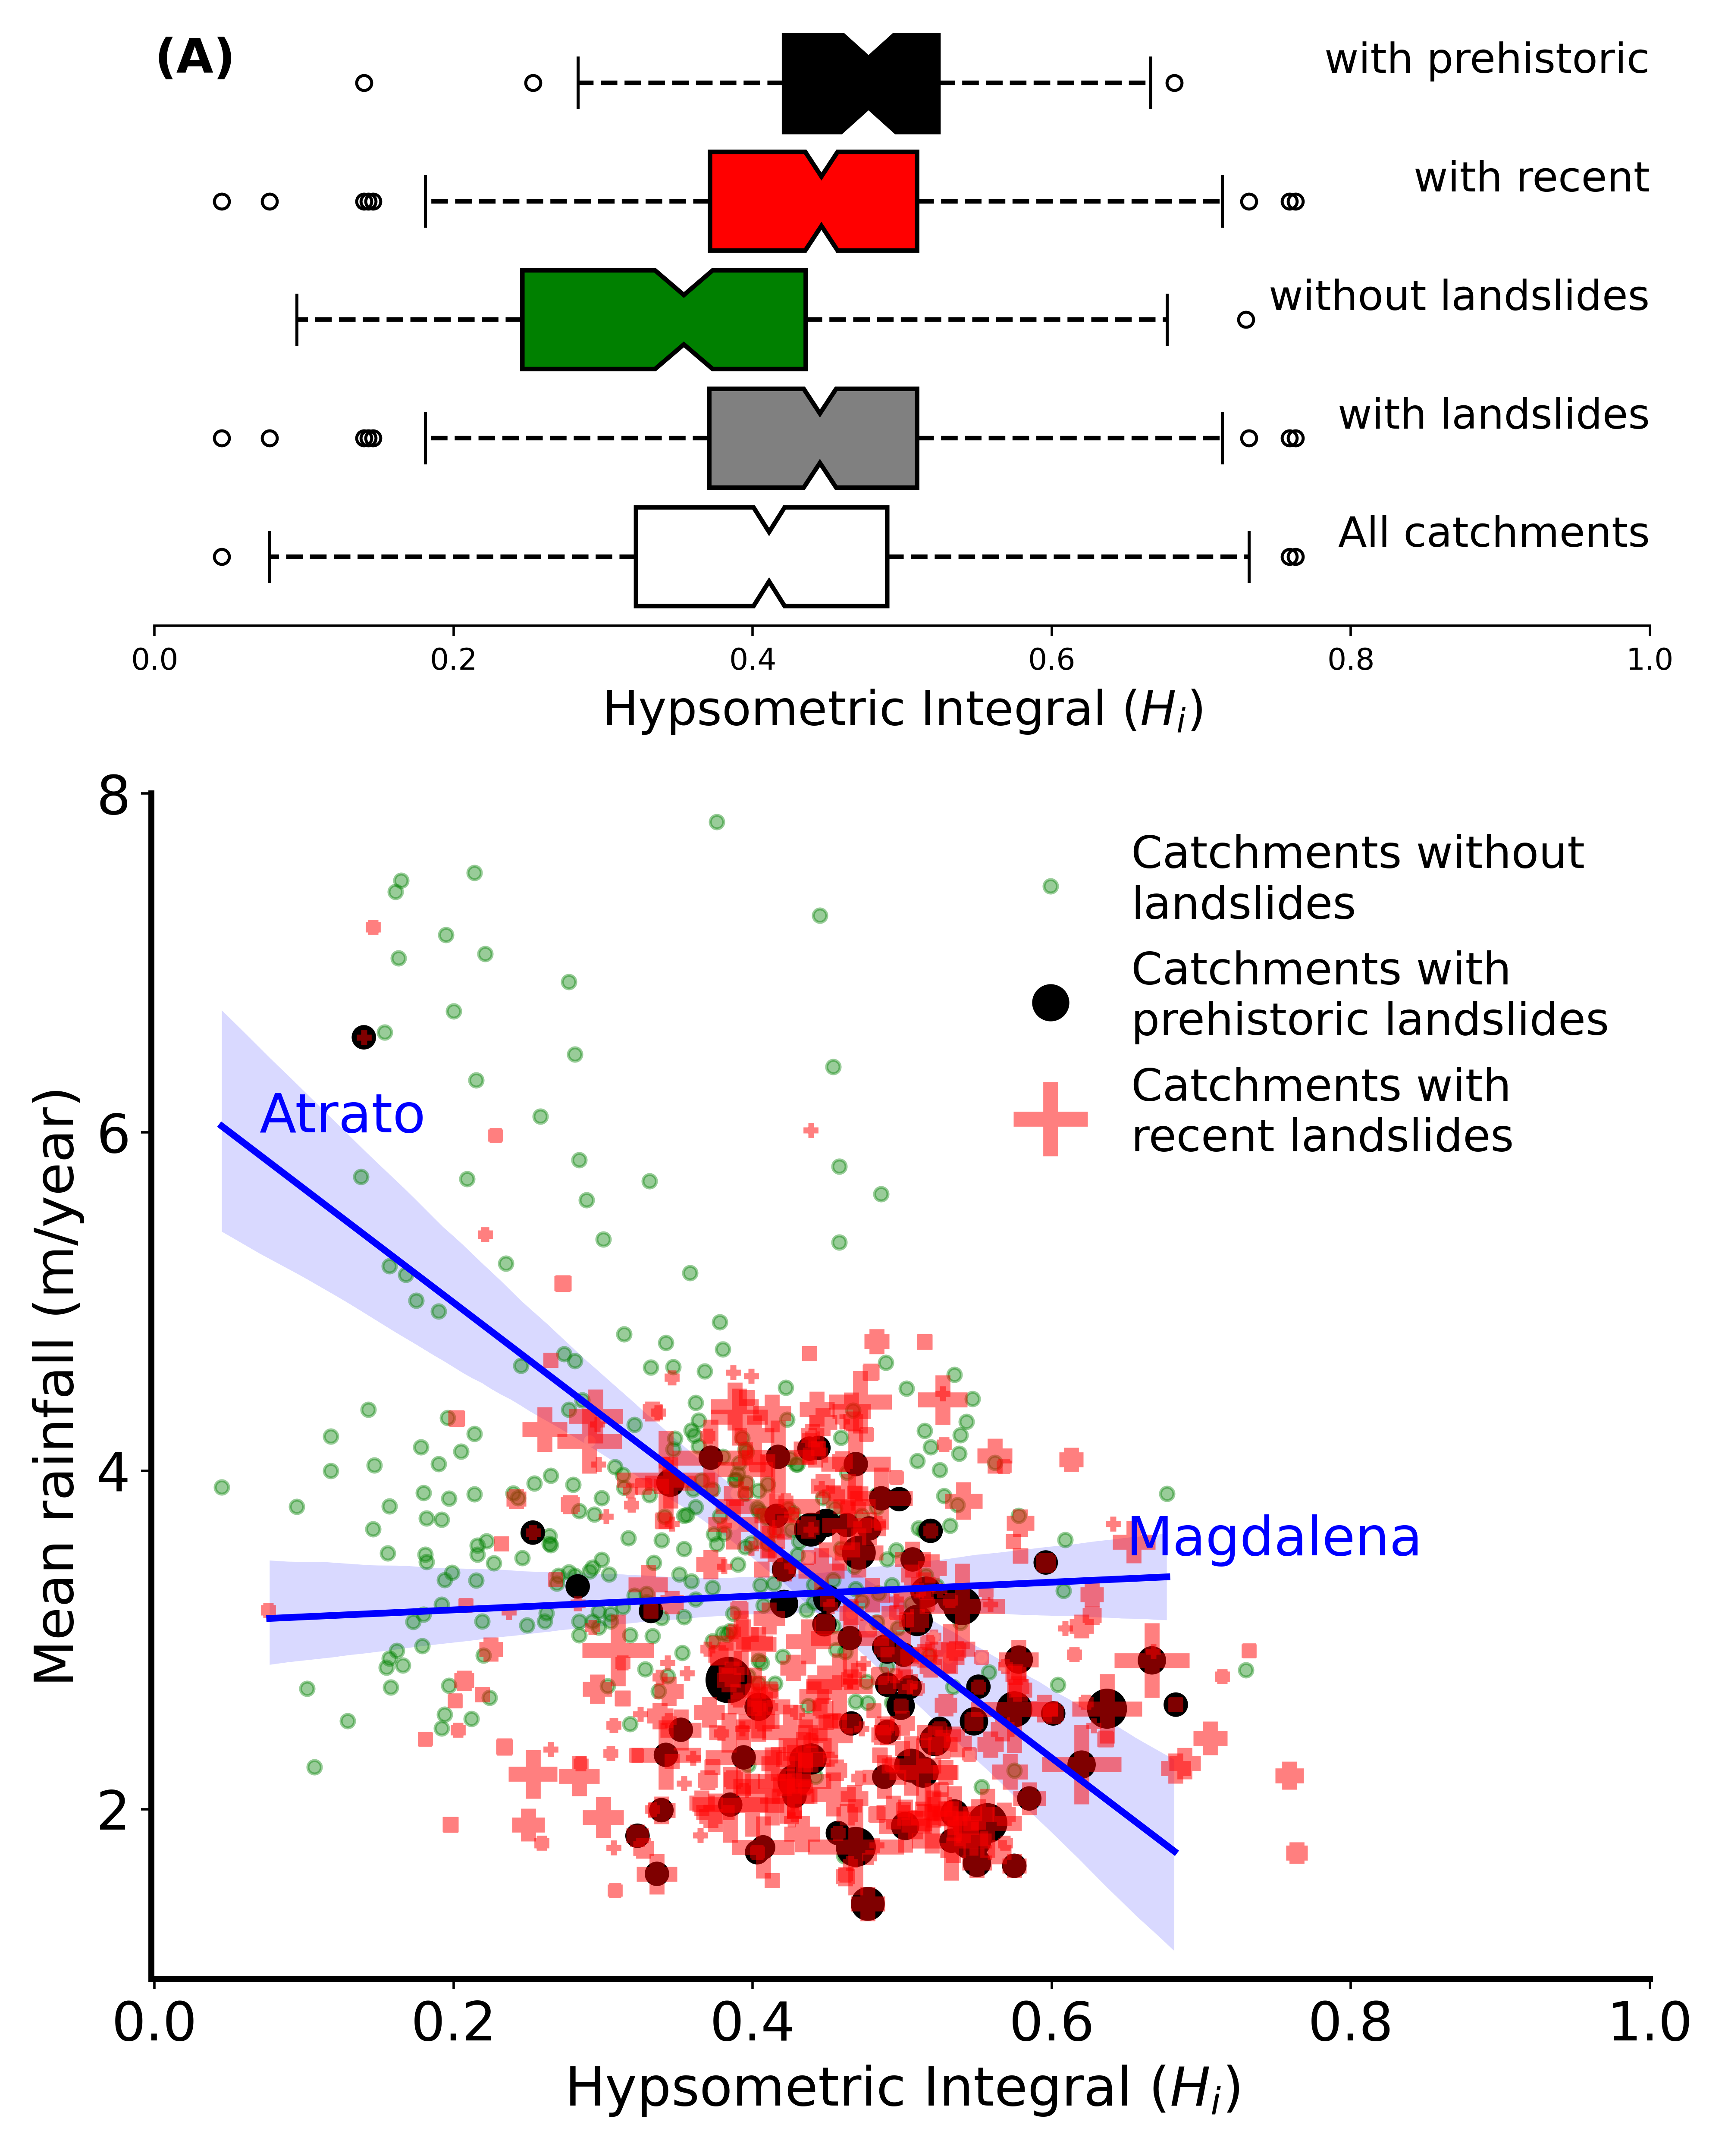
\includegraphics[width=1\textwidth]{Fig6A.png}}
  \end{minipage}\quad
  \begin{minipage}{.48\linewidth}
    \centering
%      {\includegraphics[width=1\textwidth]{Fig6B.png}}
  \end{minipage} 
    \caption{(A) Scatter plot of mean annual rainfall versus \textit{HI} averaged for each of 650 catchments with corresponding box-and-whiskers for the study area (white); catchments with landslides (gray): catchments without landslides (green); with recent landslides (red): and with prehistoric landslides (black); symbol size scaled to the number of landslide in each catchment. Box-and-whisker plots show distributions of \textit{HI}. Blue lines (and shades) are simple linear regression curves (and 95\% confidence intervals) for Atrato and Magdalena basins. (B) Catchment-wide distribution of \textit{HI} with superimposed landslide pattern.}
    \label{fig:hypso}
\end{figure}


\begin{figure}[ht!]
  \begin{minipage}{.66\linewidth}
    \centering
%      {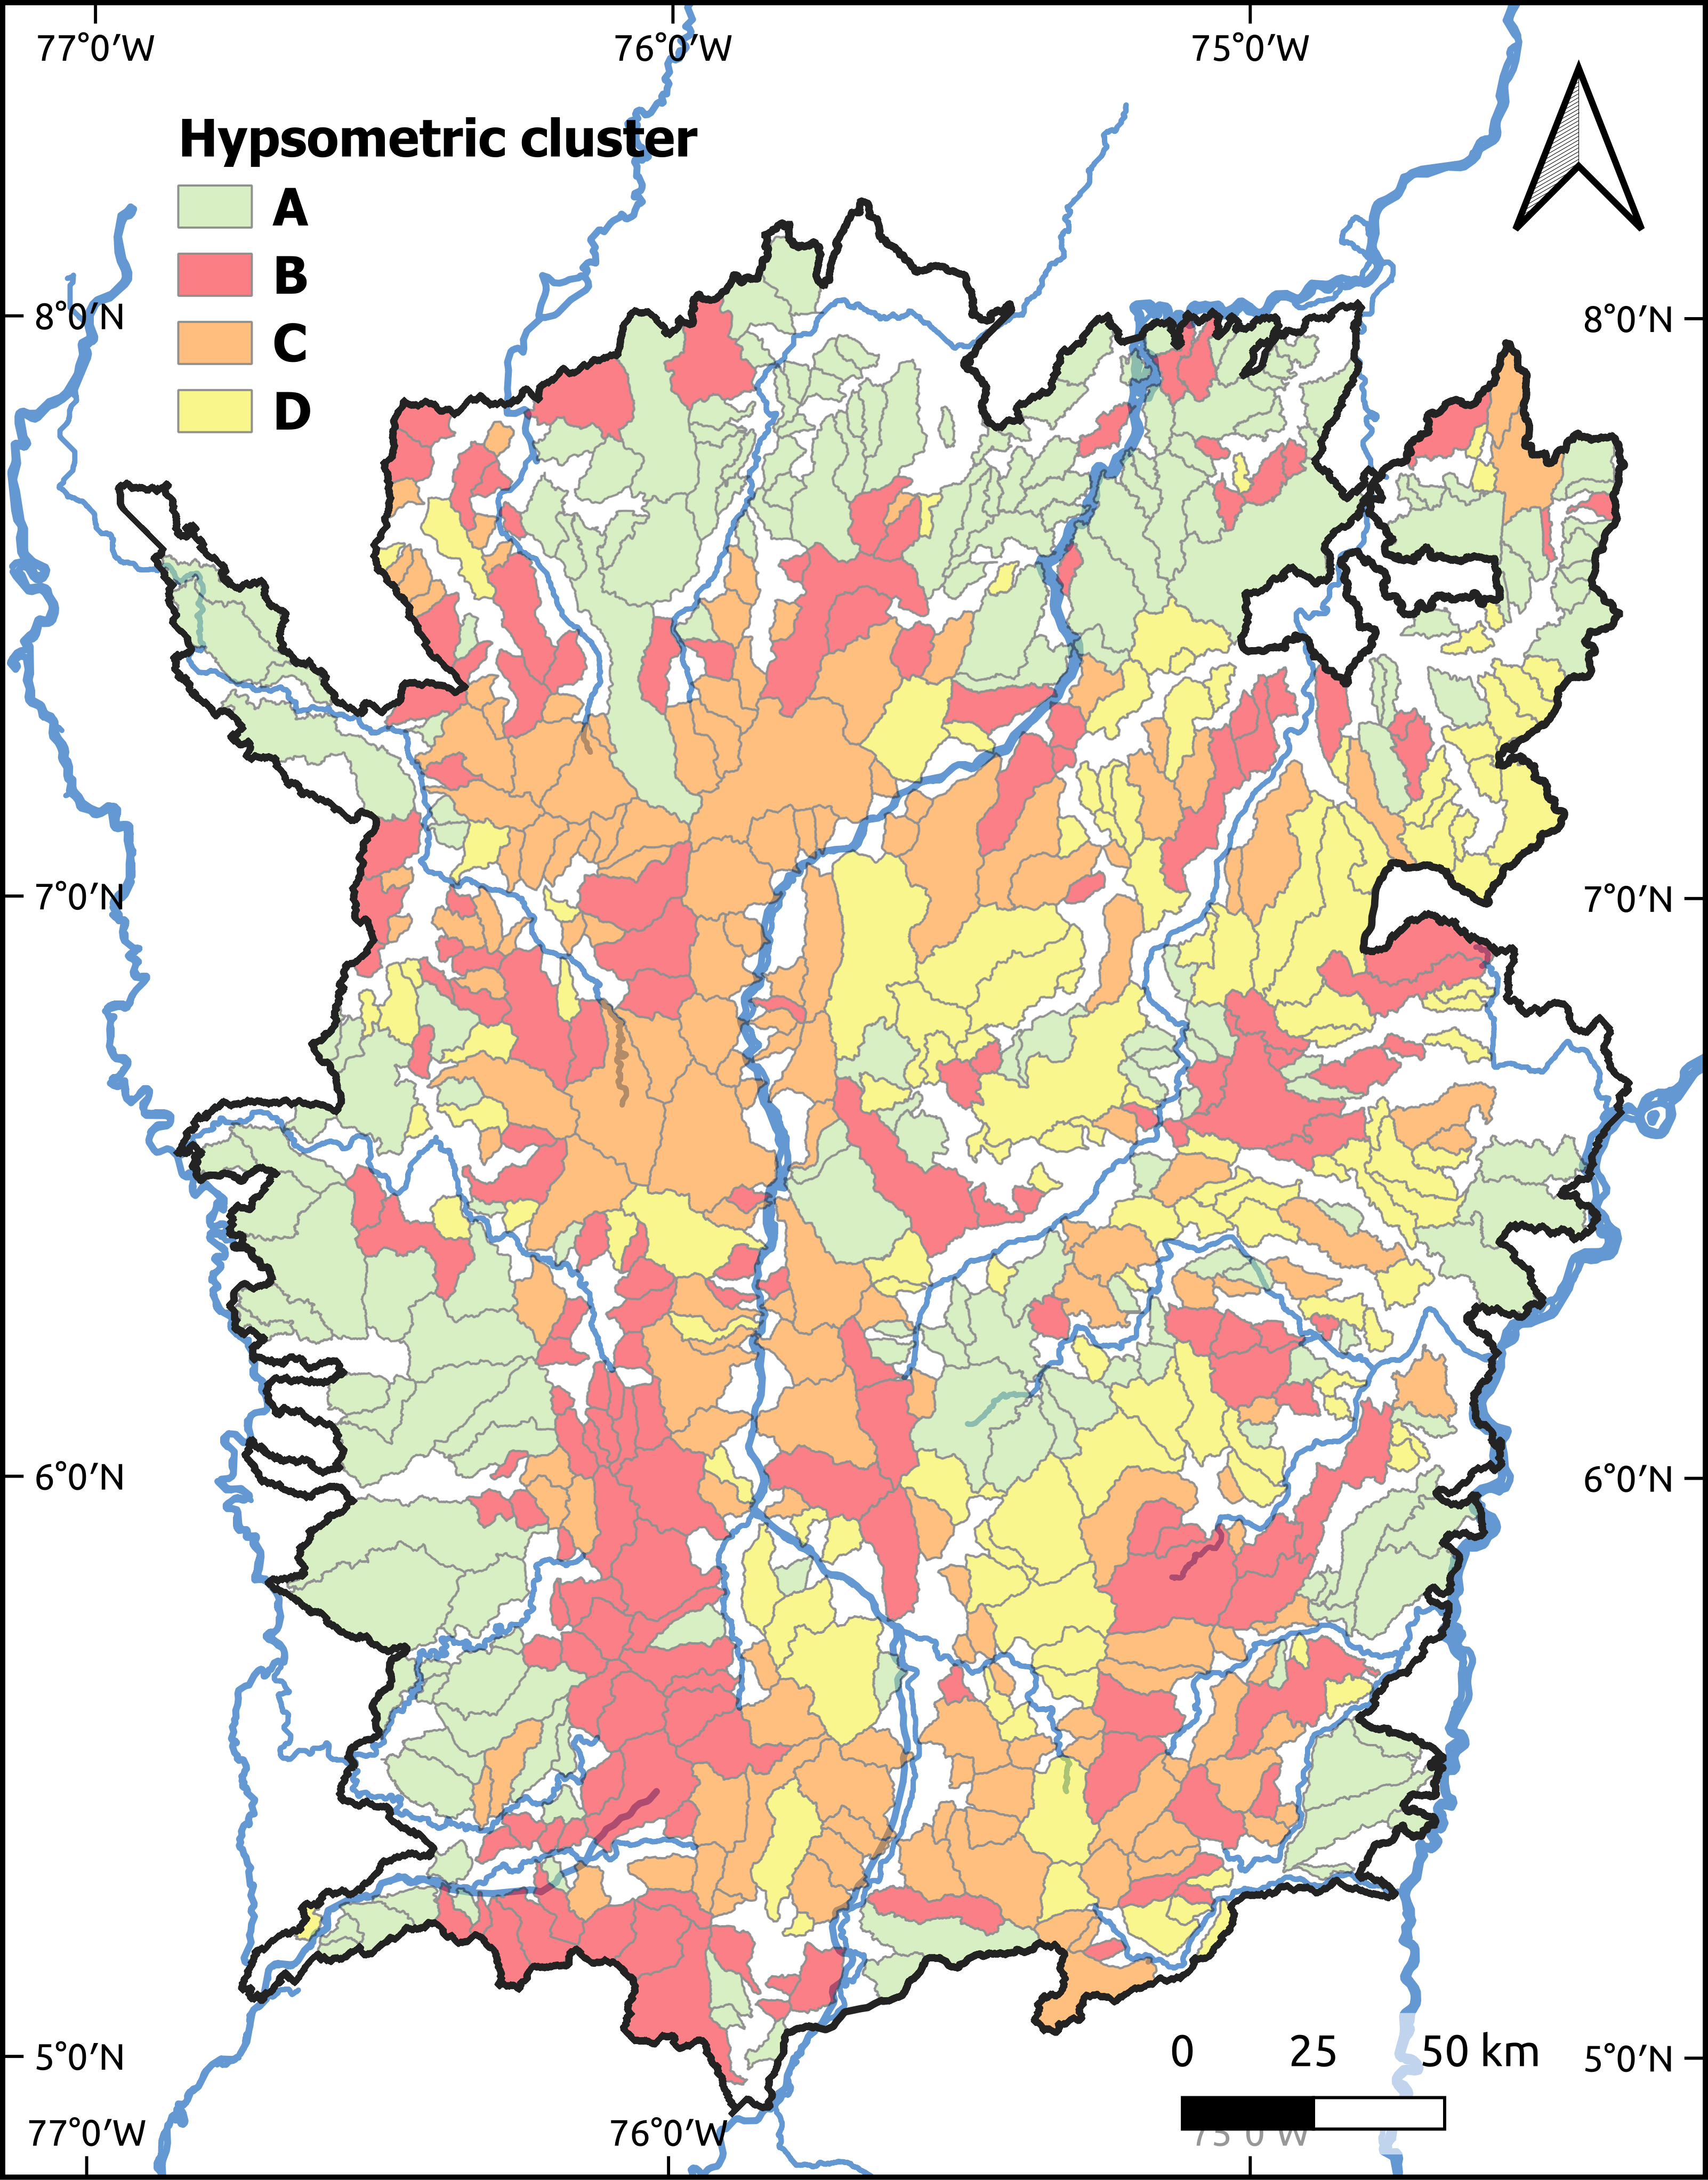
\includegraphics[width=1\textwidth]{Fig7A.png}}
  \end{minipage}\quad
  \begin{minipage}{.24\linewidth}
    \centering
%      {\includegraphics[width=1\textwidth]{Fig7B.png}}
  \end{minipage}
    \caption{$K$-means cluster analysis of catchment hypsometry reveals four distinct groups (A-D) of catchments (left) with differing distributions of normalized elevation (color-coded lines, right; grey lines are raw data for each catchment). Clusters A to D identify groups of catchments with shifting dominance from lower to higher relative elevations.}
    \label{fig:knickpoints}
\end{figure}

\begin{figure}[ht!]
%     {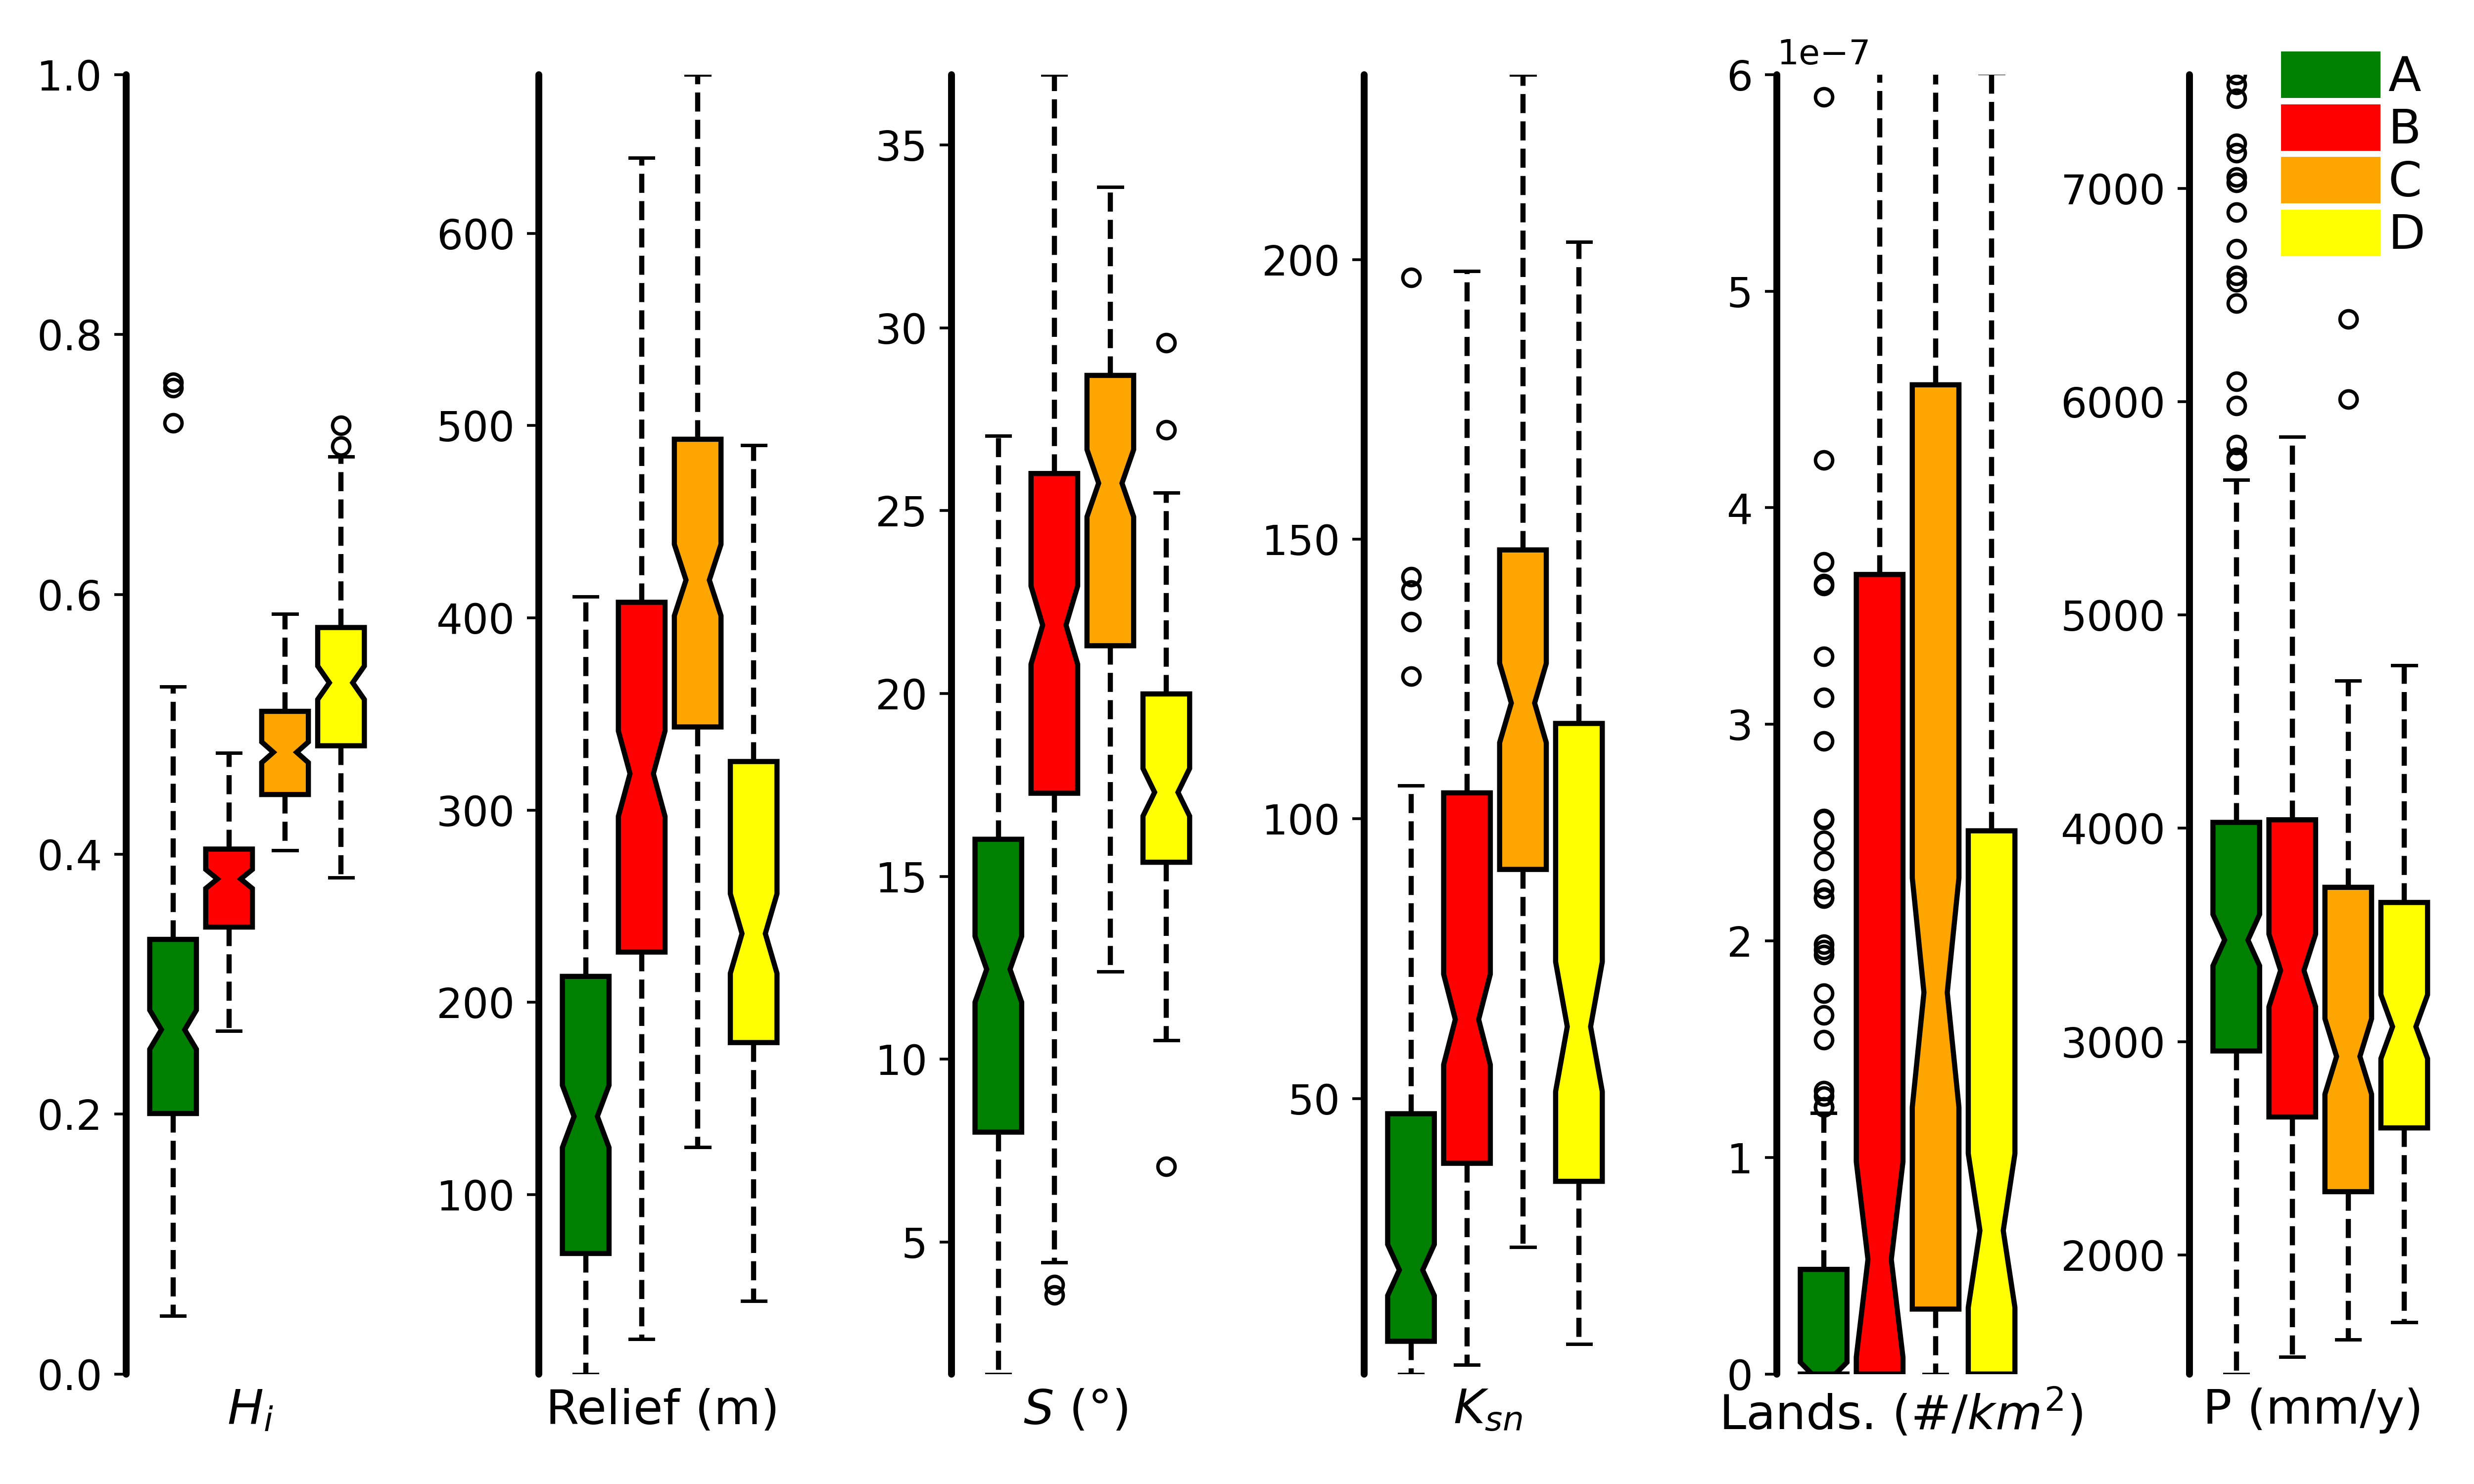
\includegraphics[width=1\textwidth]{Fig8.png}}
    \caption{Distributions of catchment-averaged topographic metrics, i.e. hypsometric integral $HI$, relief, slope, landslide density (Lands.), and mean annual rainfall $P$ for each hypsometric cluster (Fig.~\ref{fig:knickpoints}). Box-and-whisker plots show medians with notches (95\% confidence Interval); whiskers span 1.5~times the interquartile range; bubbles are outside this range. Note how the distributions of these metrics differ between clusters (A, B, C and D) without having been part of the original cluster derivation.}
  \label{fig:cluster2}
\end{figure}

\begin{figure}[ht!]
  \begin{minipage}{.48\linewidth}
    \centering
%      {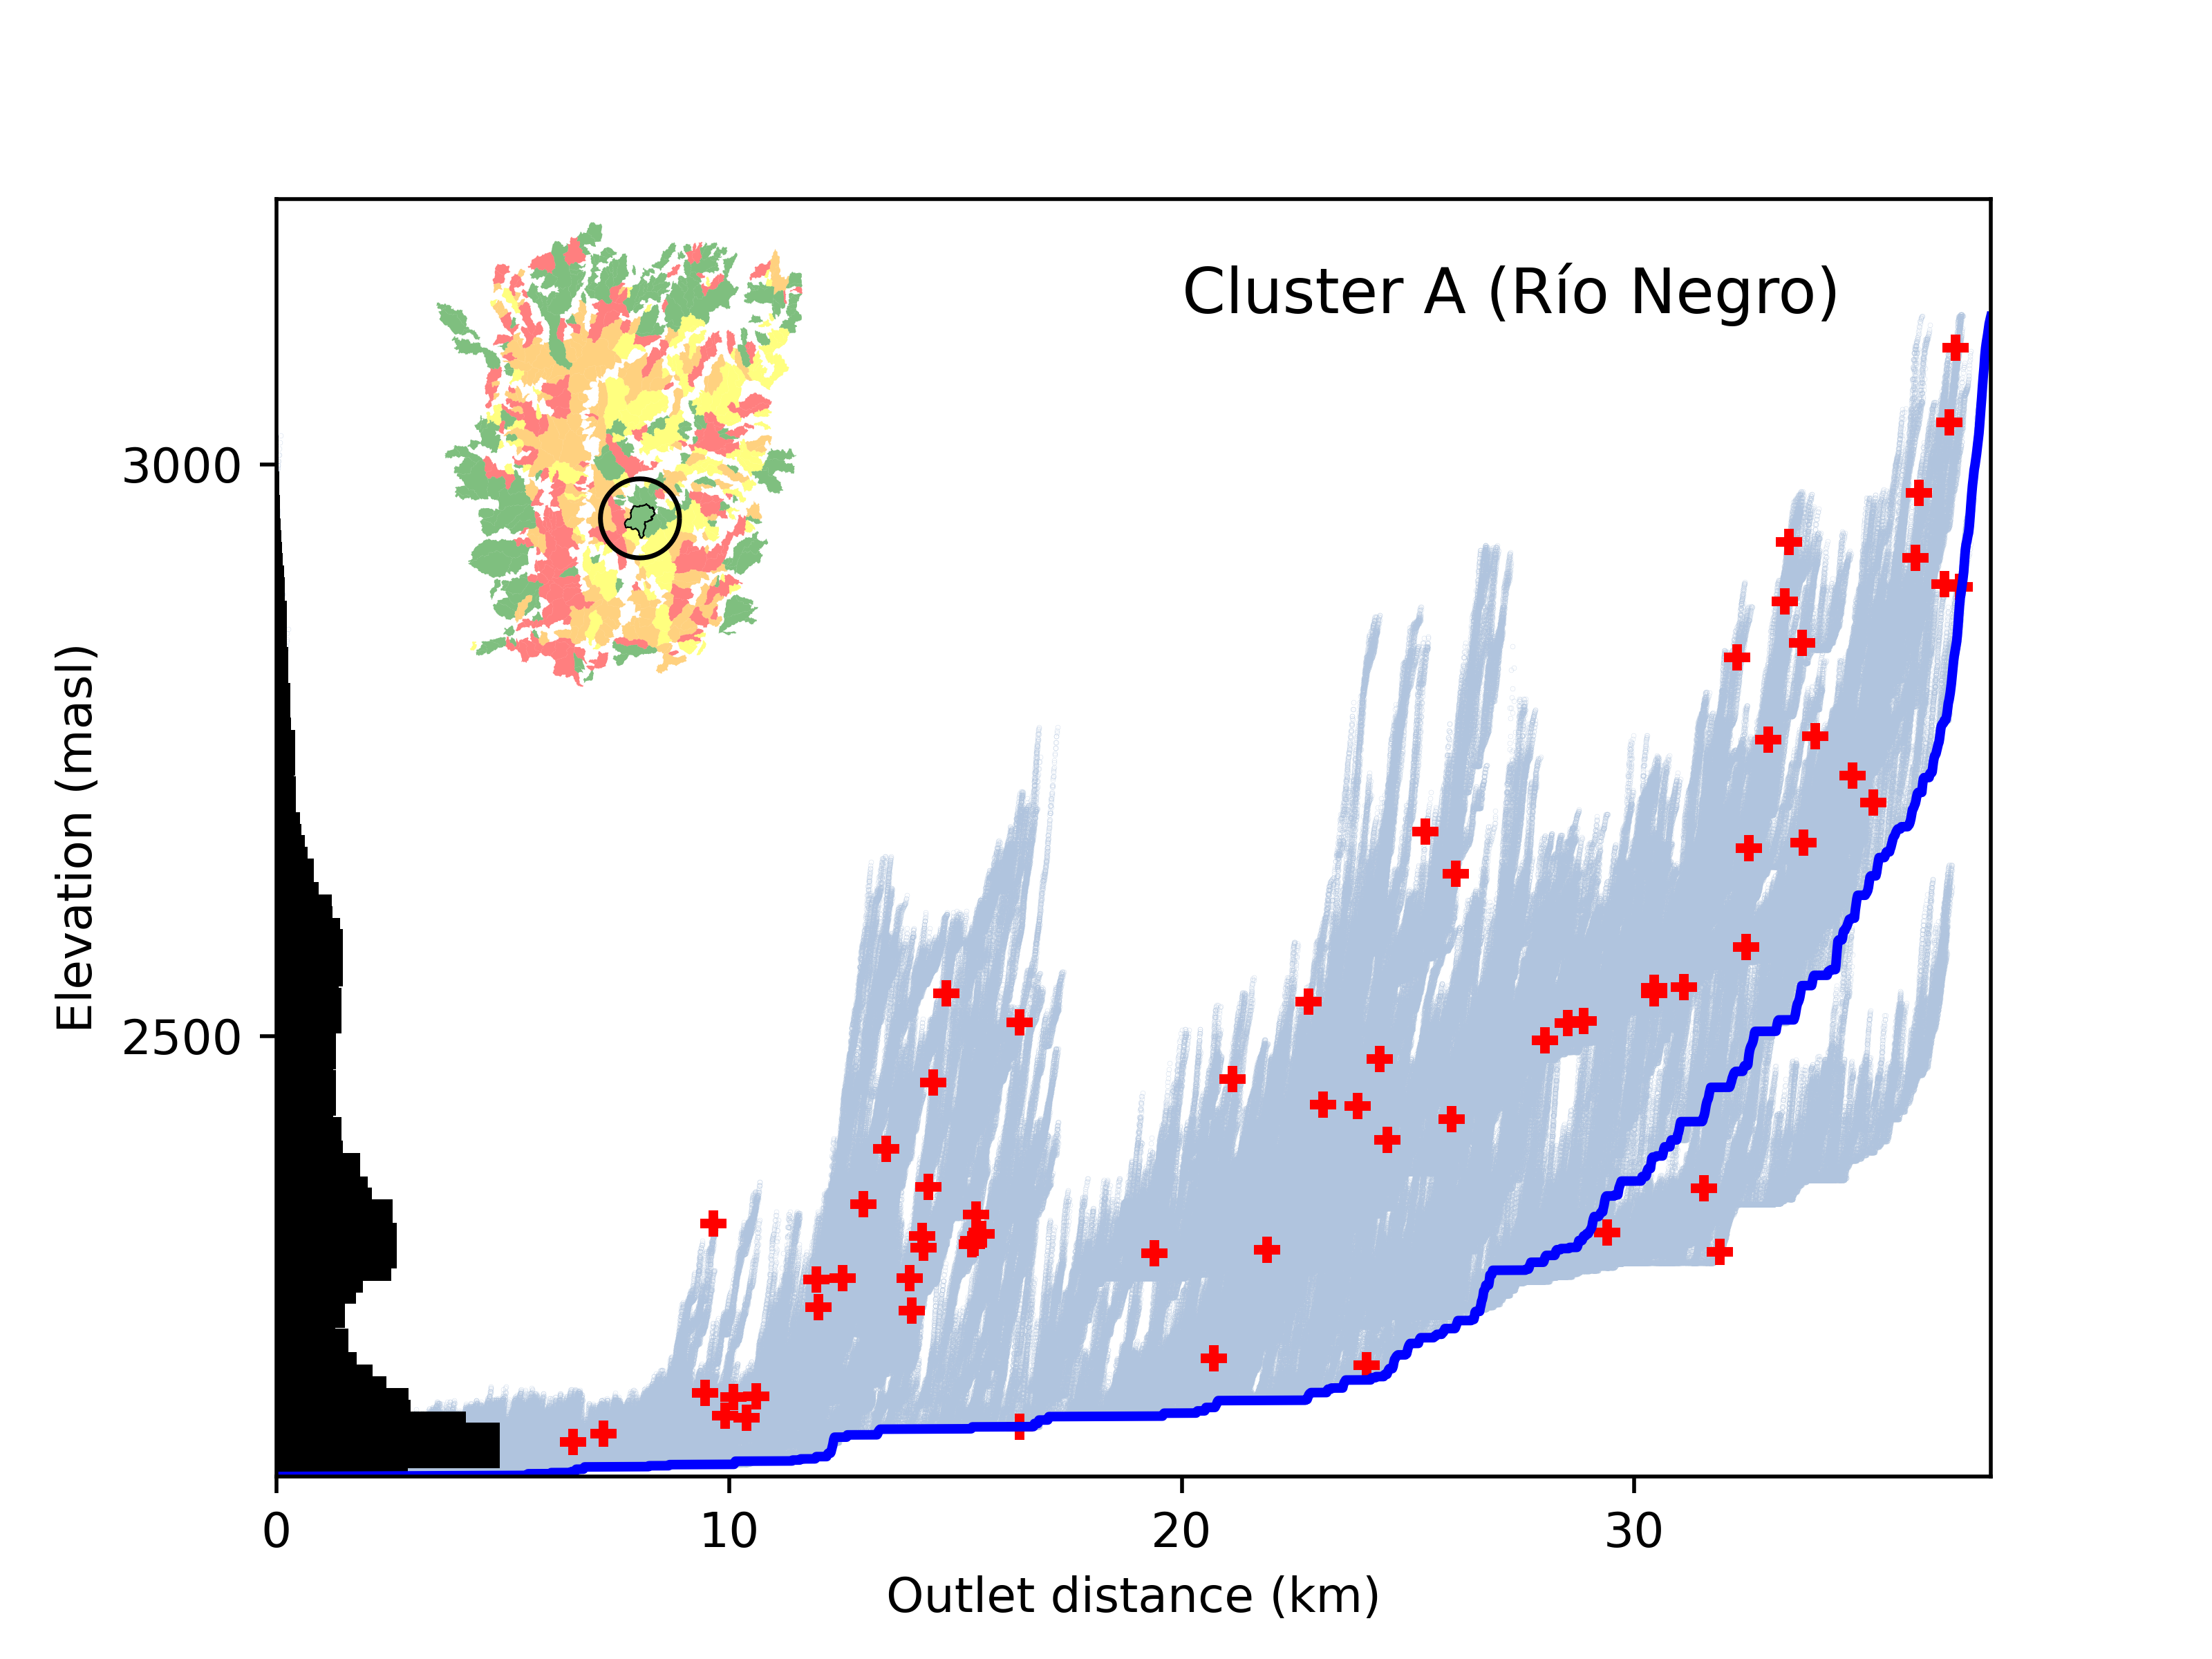
\includegraphics[width=1\textwidth]{Fig9A.png}}
%      {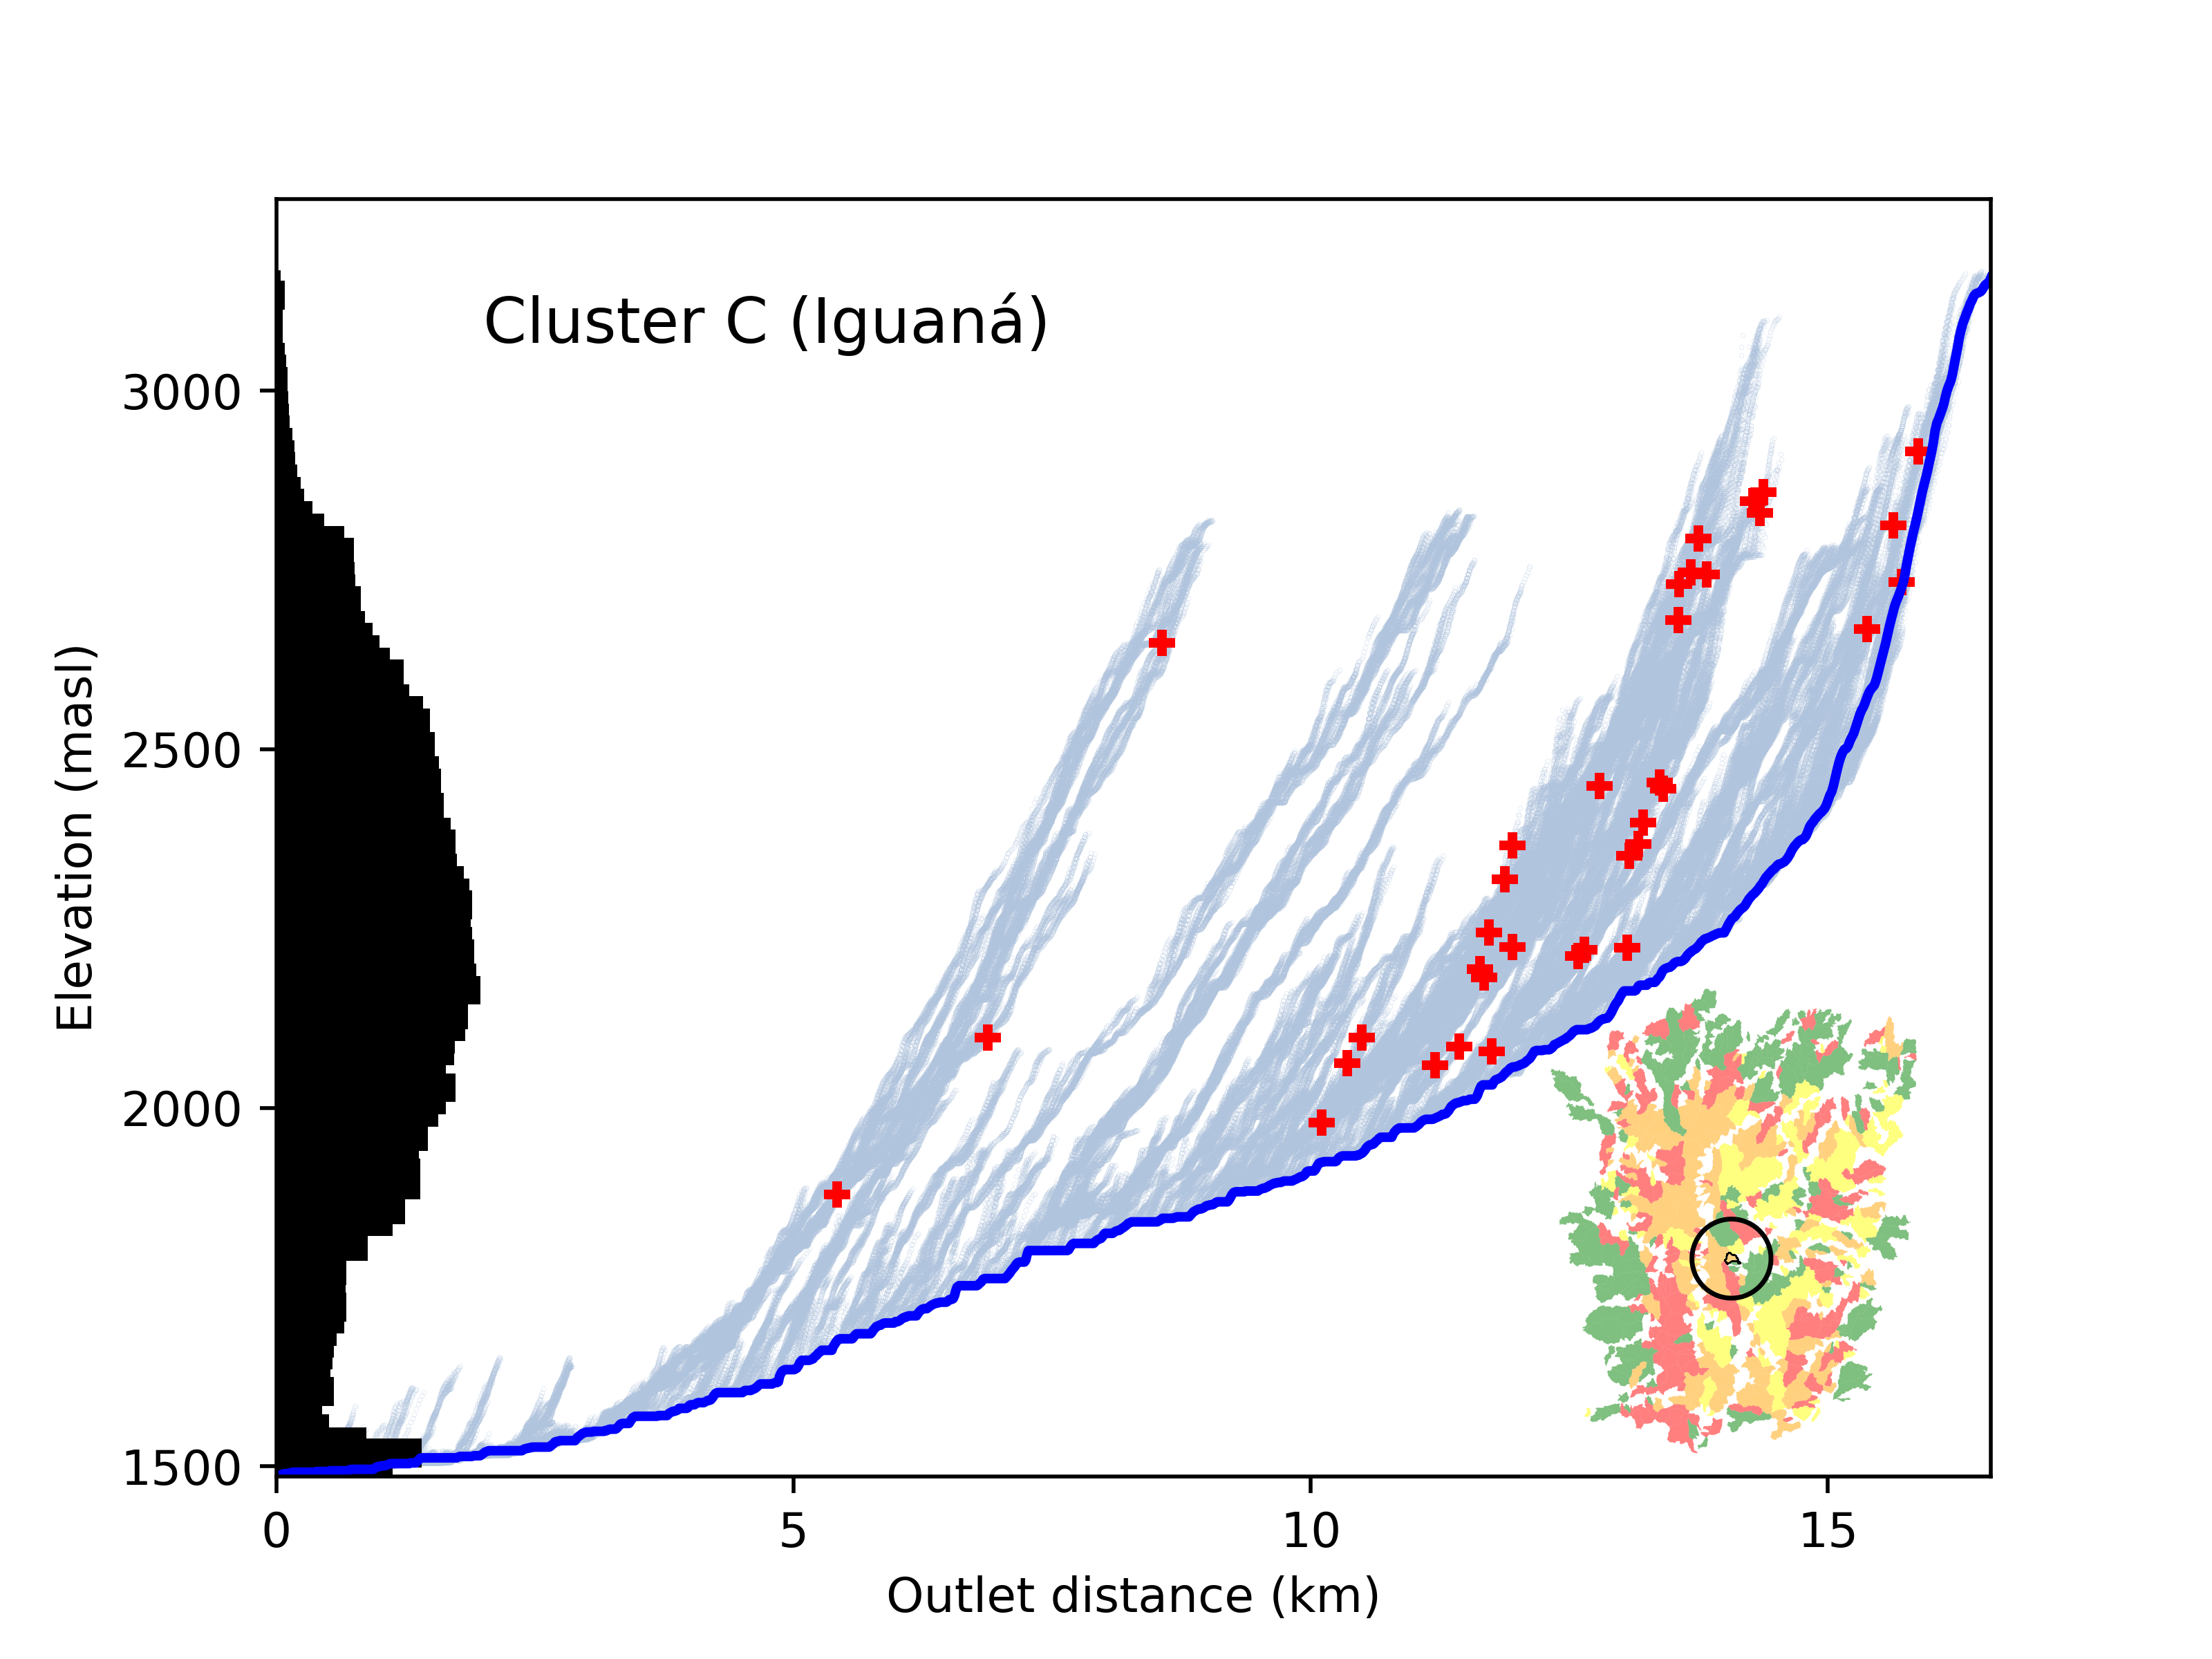
\includegraphics[width=1\textwidth]{Fig9C.png}}
  \end{minipage}\quad
  \begin{minipage}{.48\linewidth}
    \centering
%      {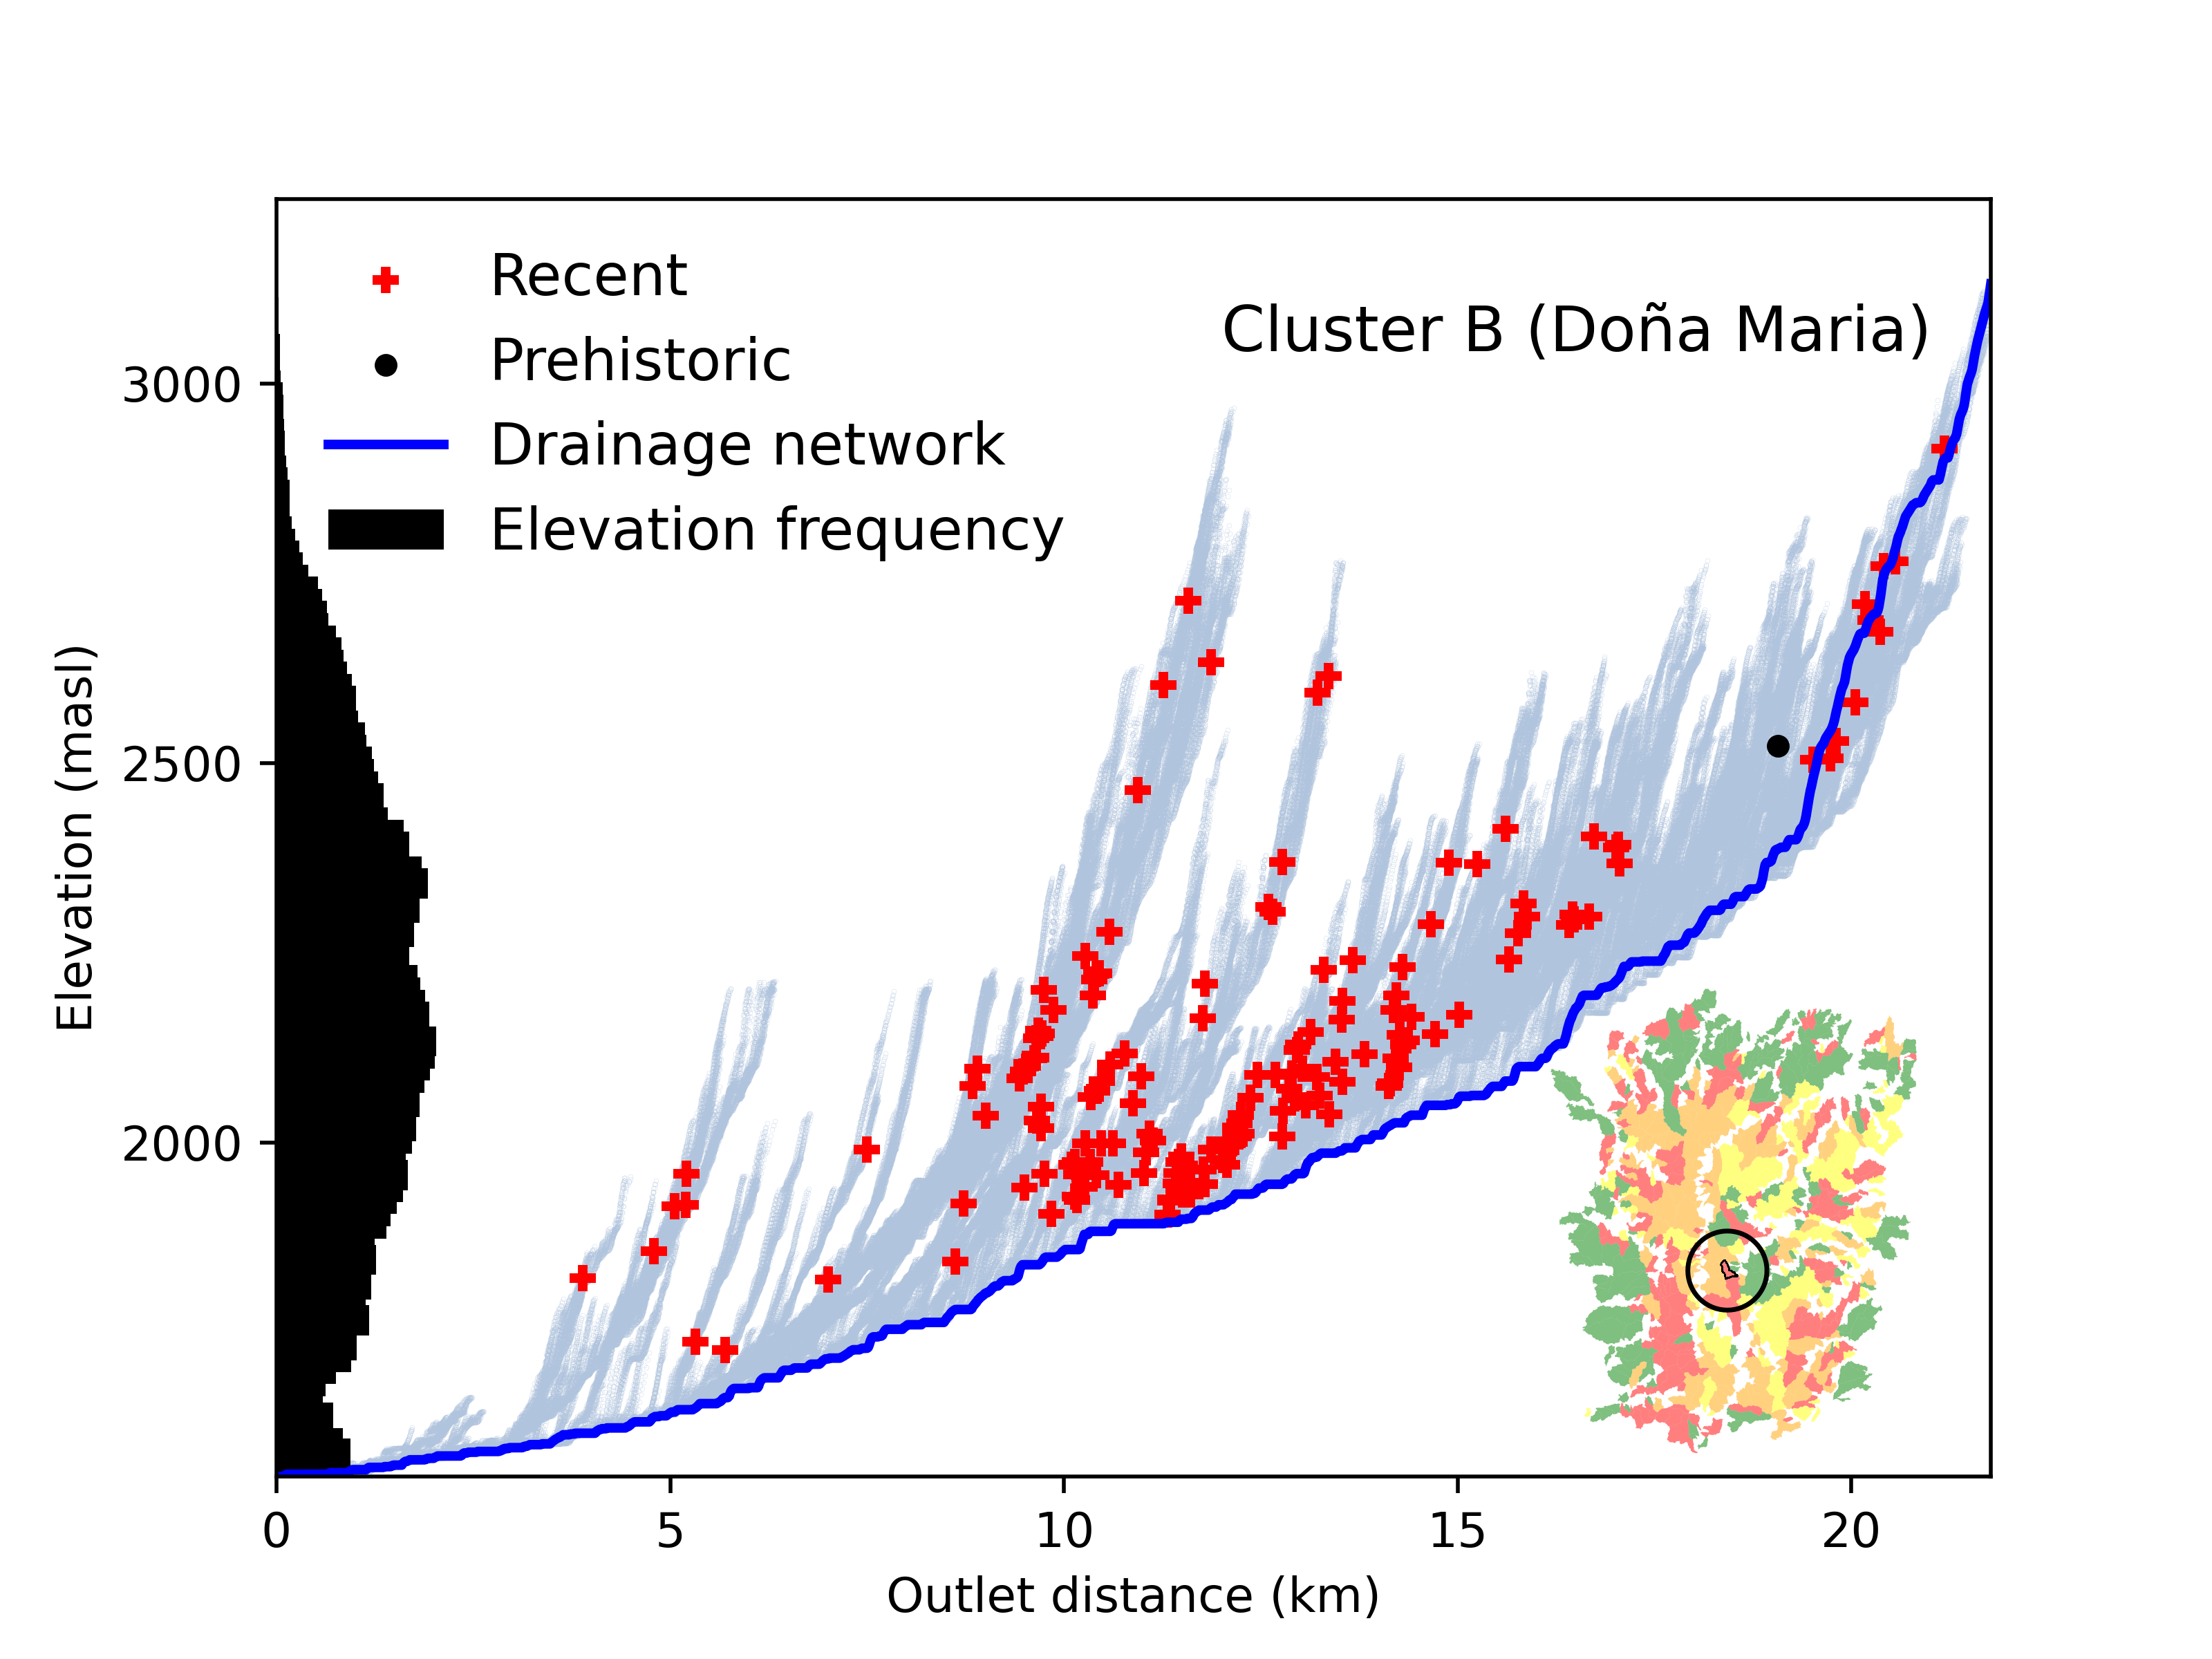
\includegraphics[width=1\textwidth]{Fig9B.png}}
%      {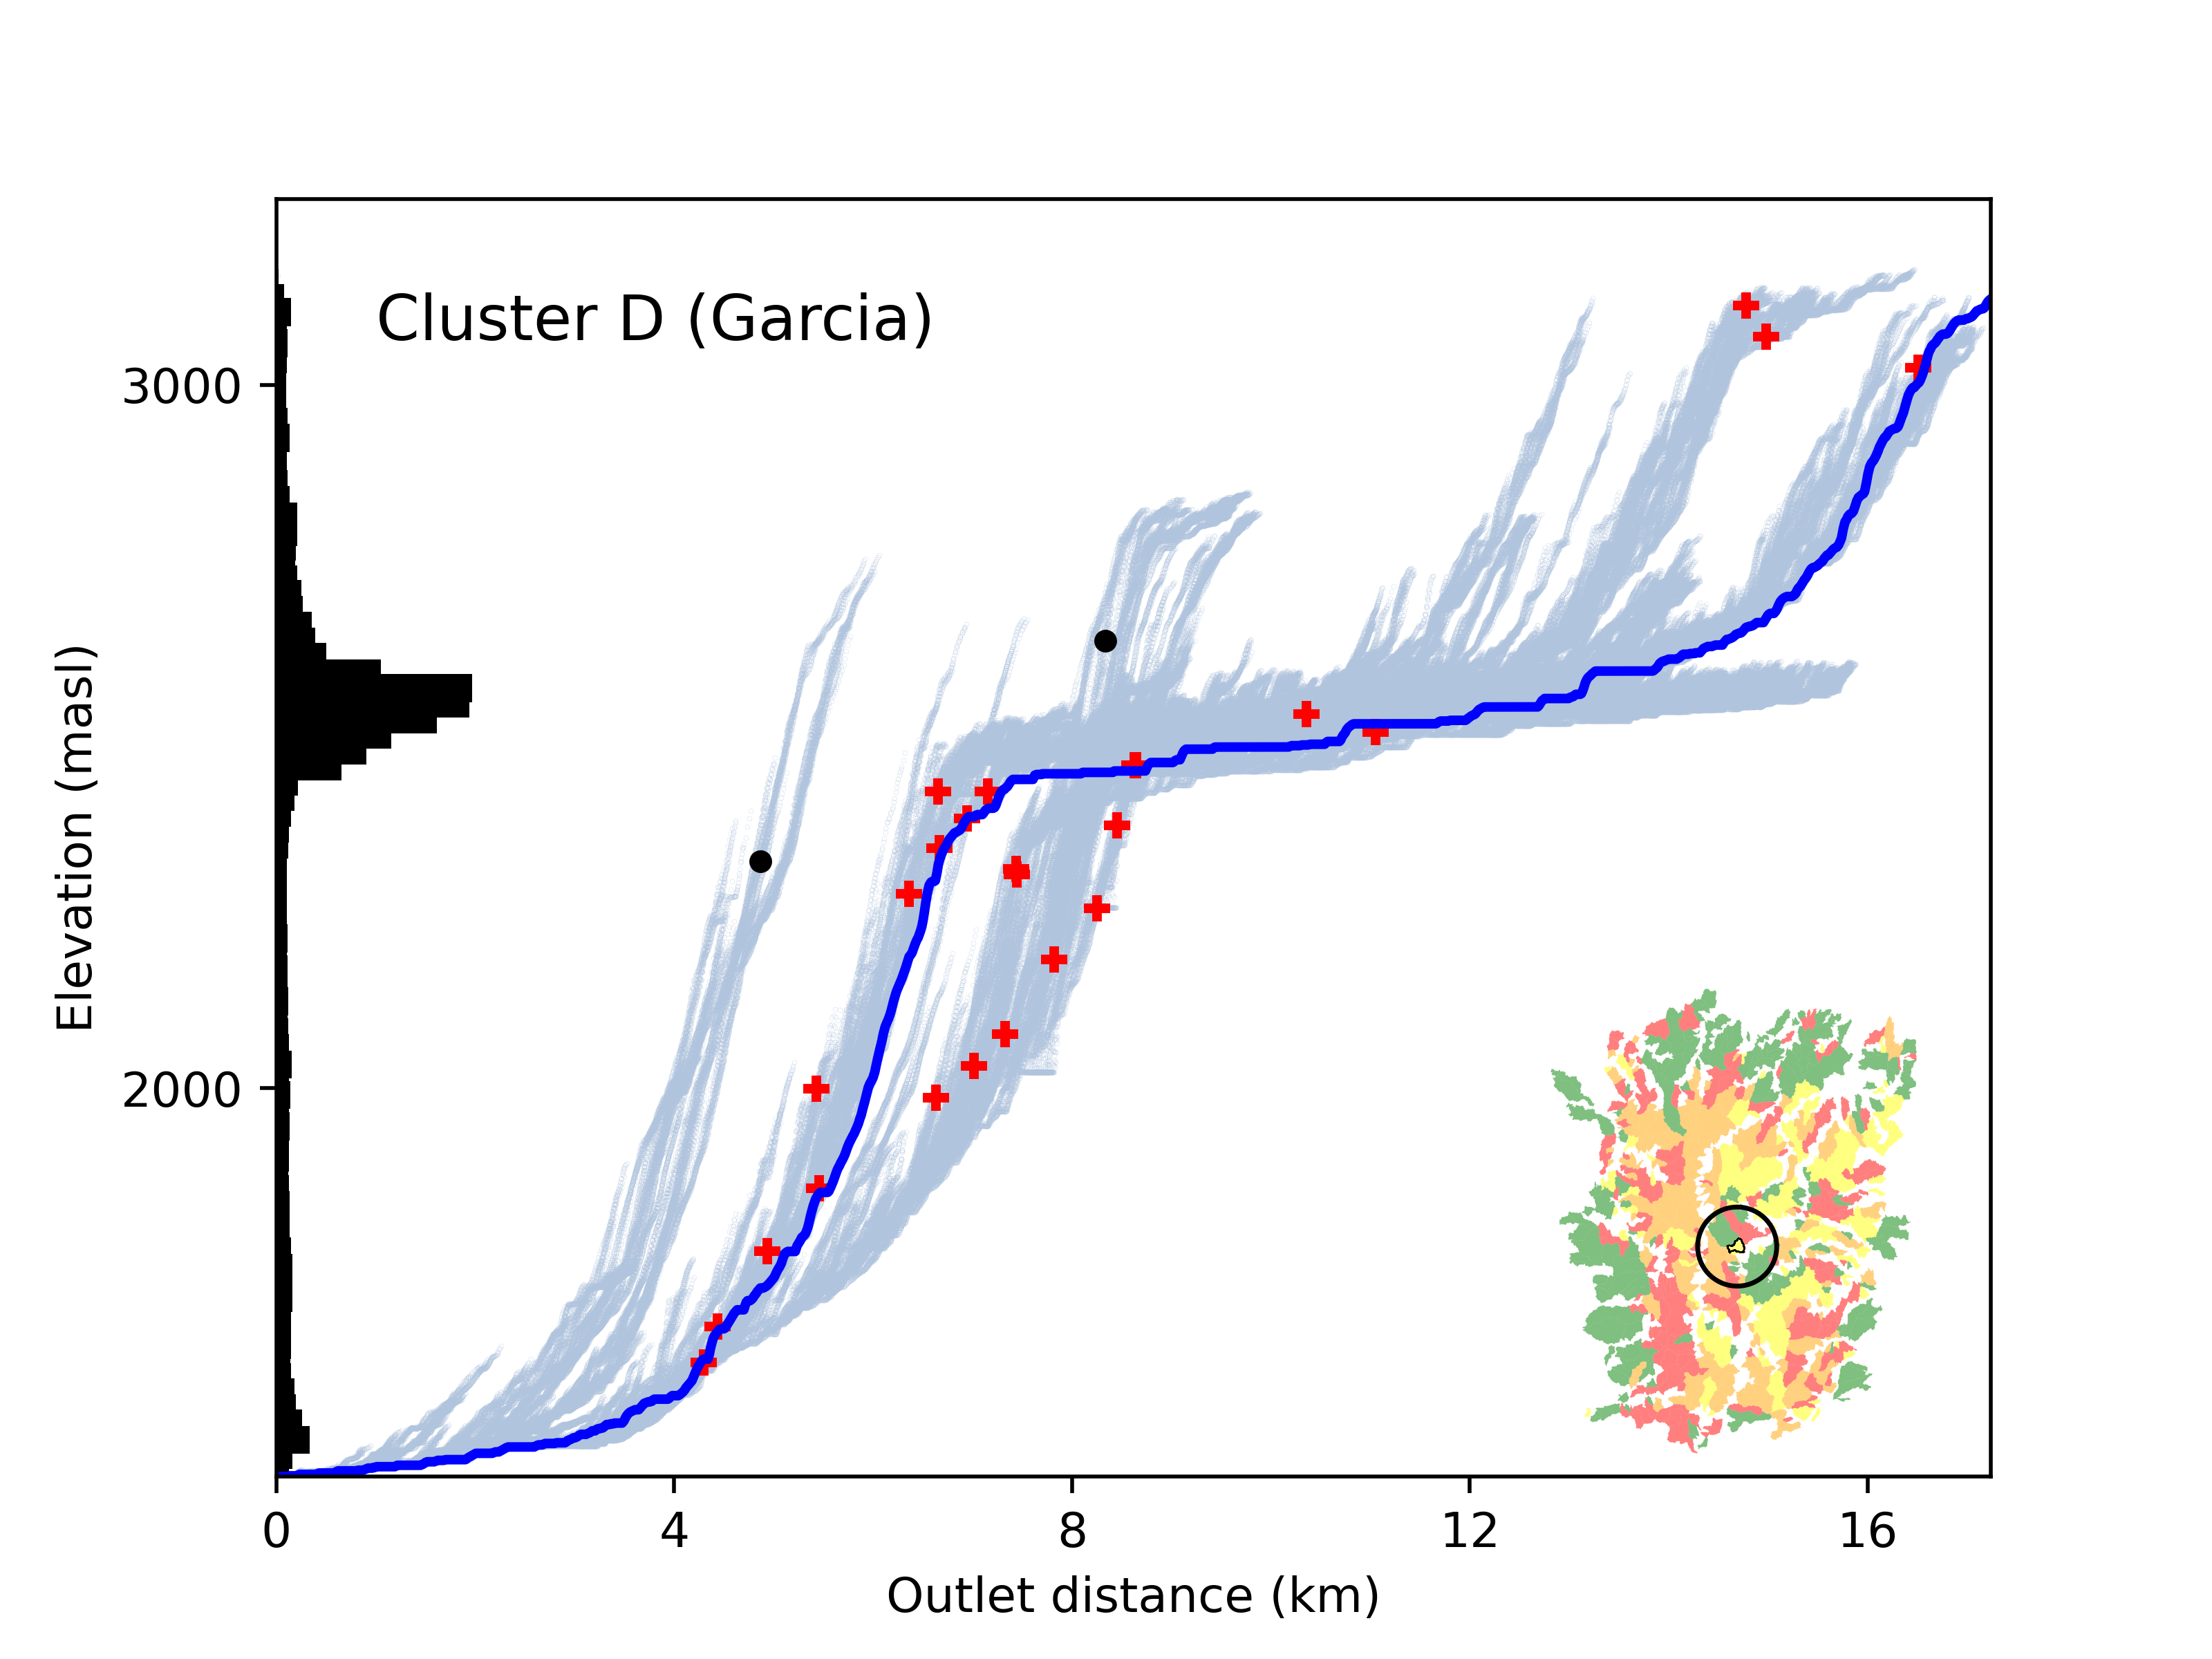
\includegraphics[width=1\textwidth]{Fig9D.png}}
  \end{minipage}
    \caption{River longitudinal profiles (blue), hypsometry (marginal histograms), and landslide distributions in sample catchments from clusters A, B, C and D each. Note the spatial proximity of the four catchments. Landslide outlet distance are projected to the closest drainage channel.}
    \label{fig:cluster-profile}
\end{figure}

\begin{figure}[ht!]
  \begin{minipage}{.48\linewidth}
    \centering
%      {\includegraphics[width=1\textwidth]{Fig10A.png}} 
%      {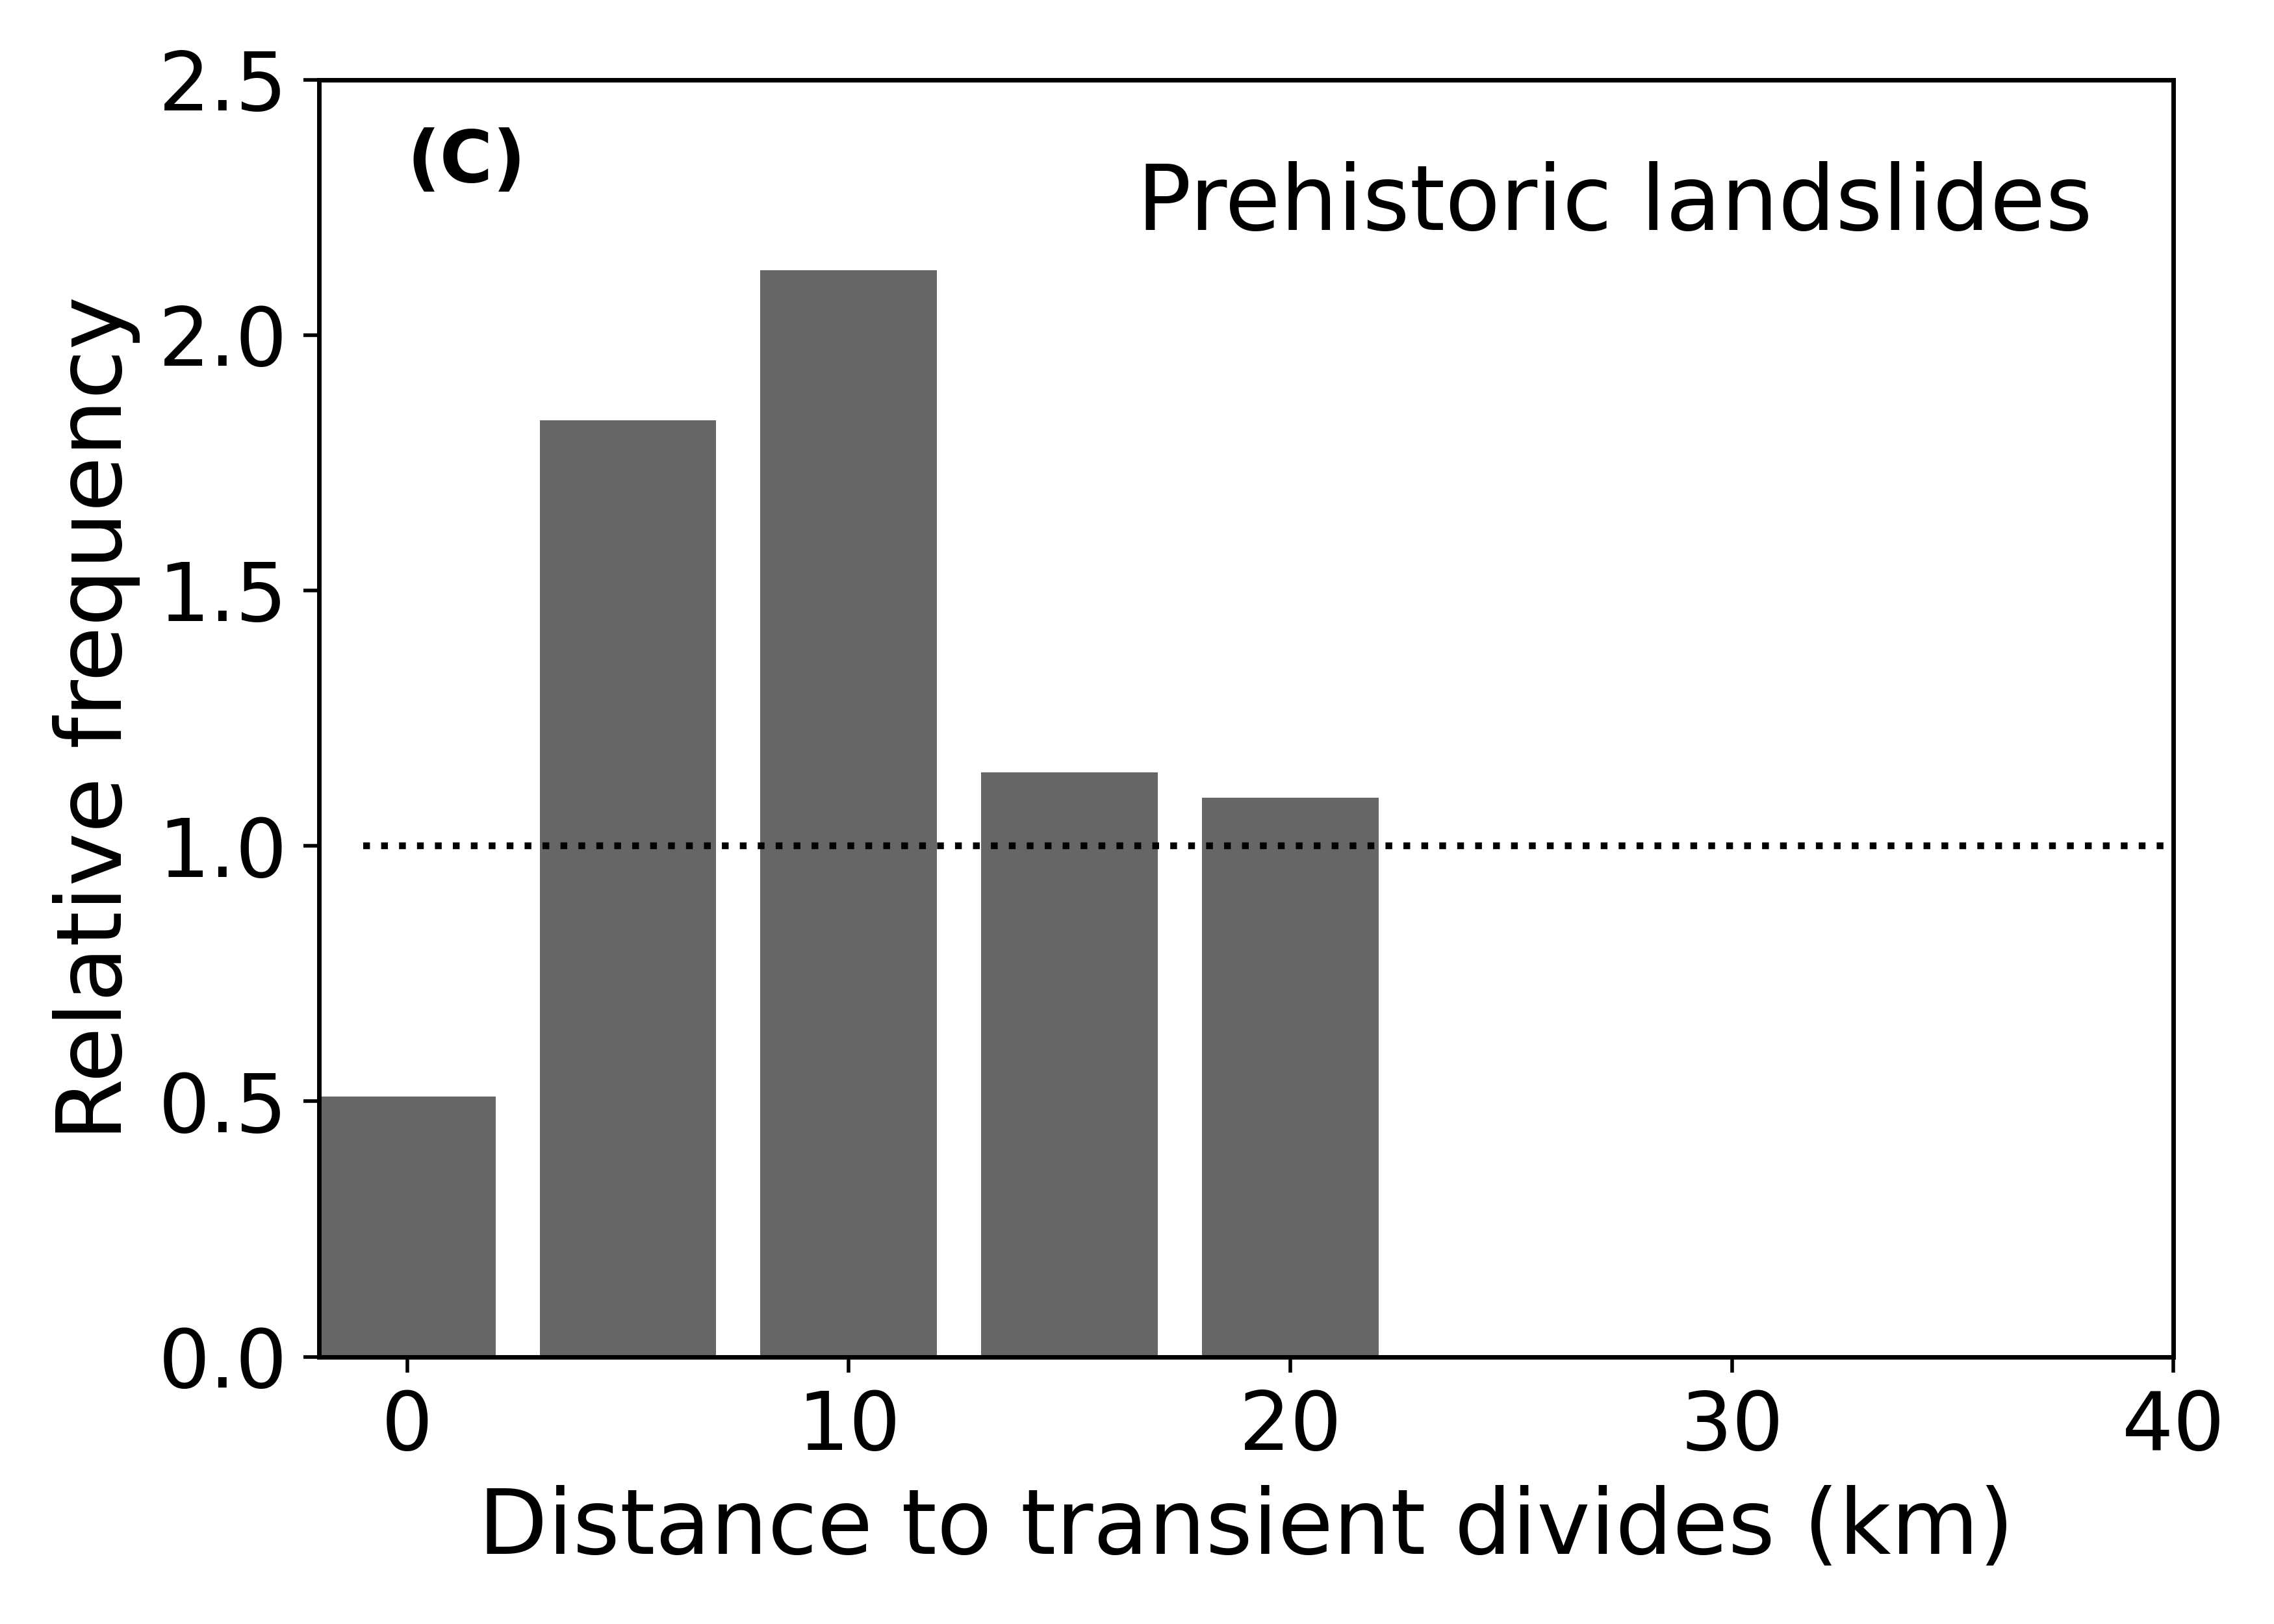
\includegraphics[width=1\textwidth]{Fig10C.png}}
  \end{minipage}\quad
  \begin{minipage}{.48\linewidth}
    \centering
%      {\includegraphics[width=1\textwidth]{Fig10B.png}}
%      {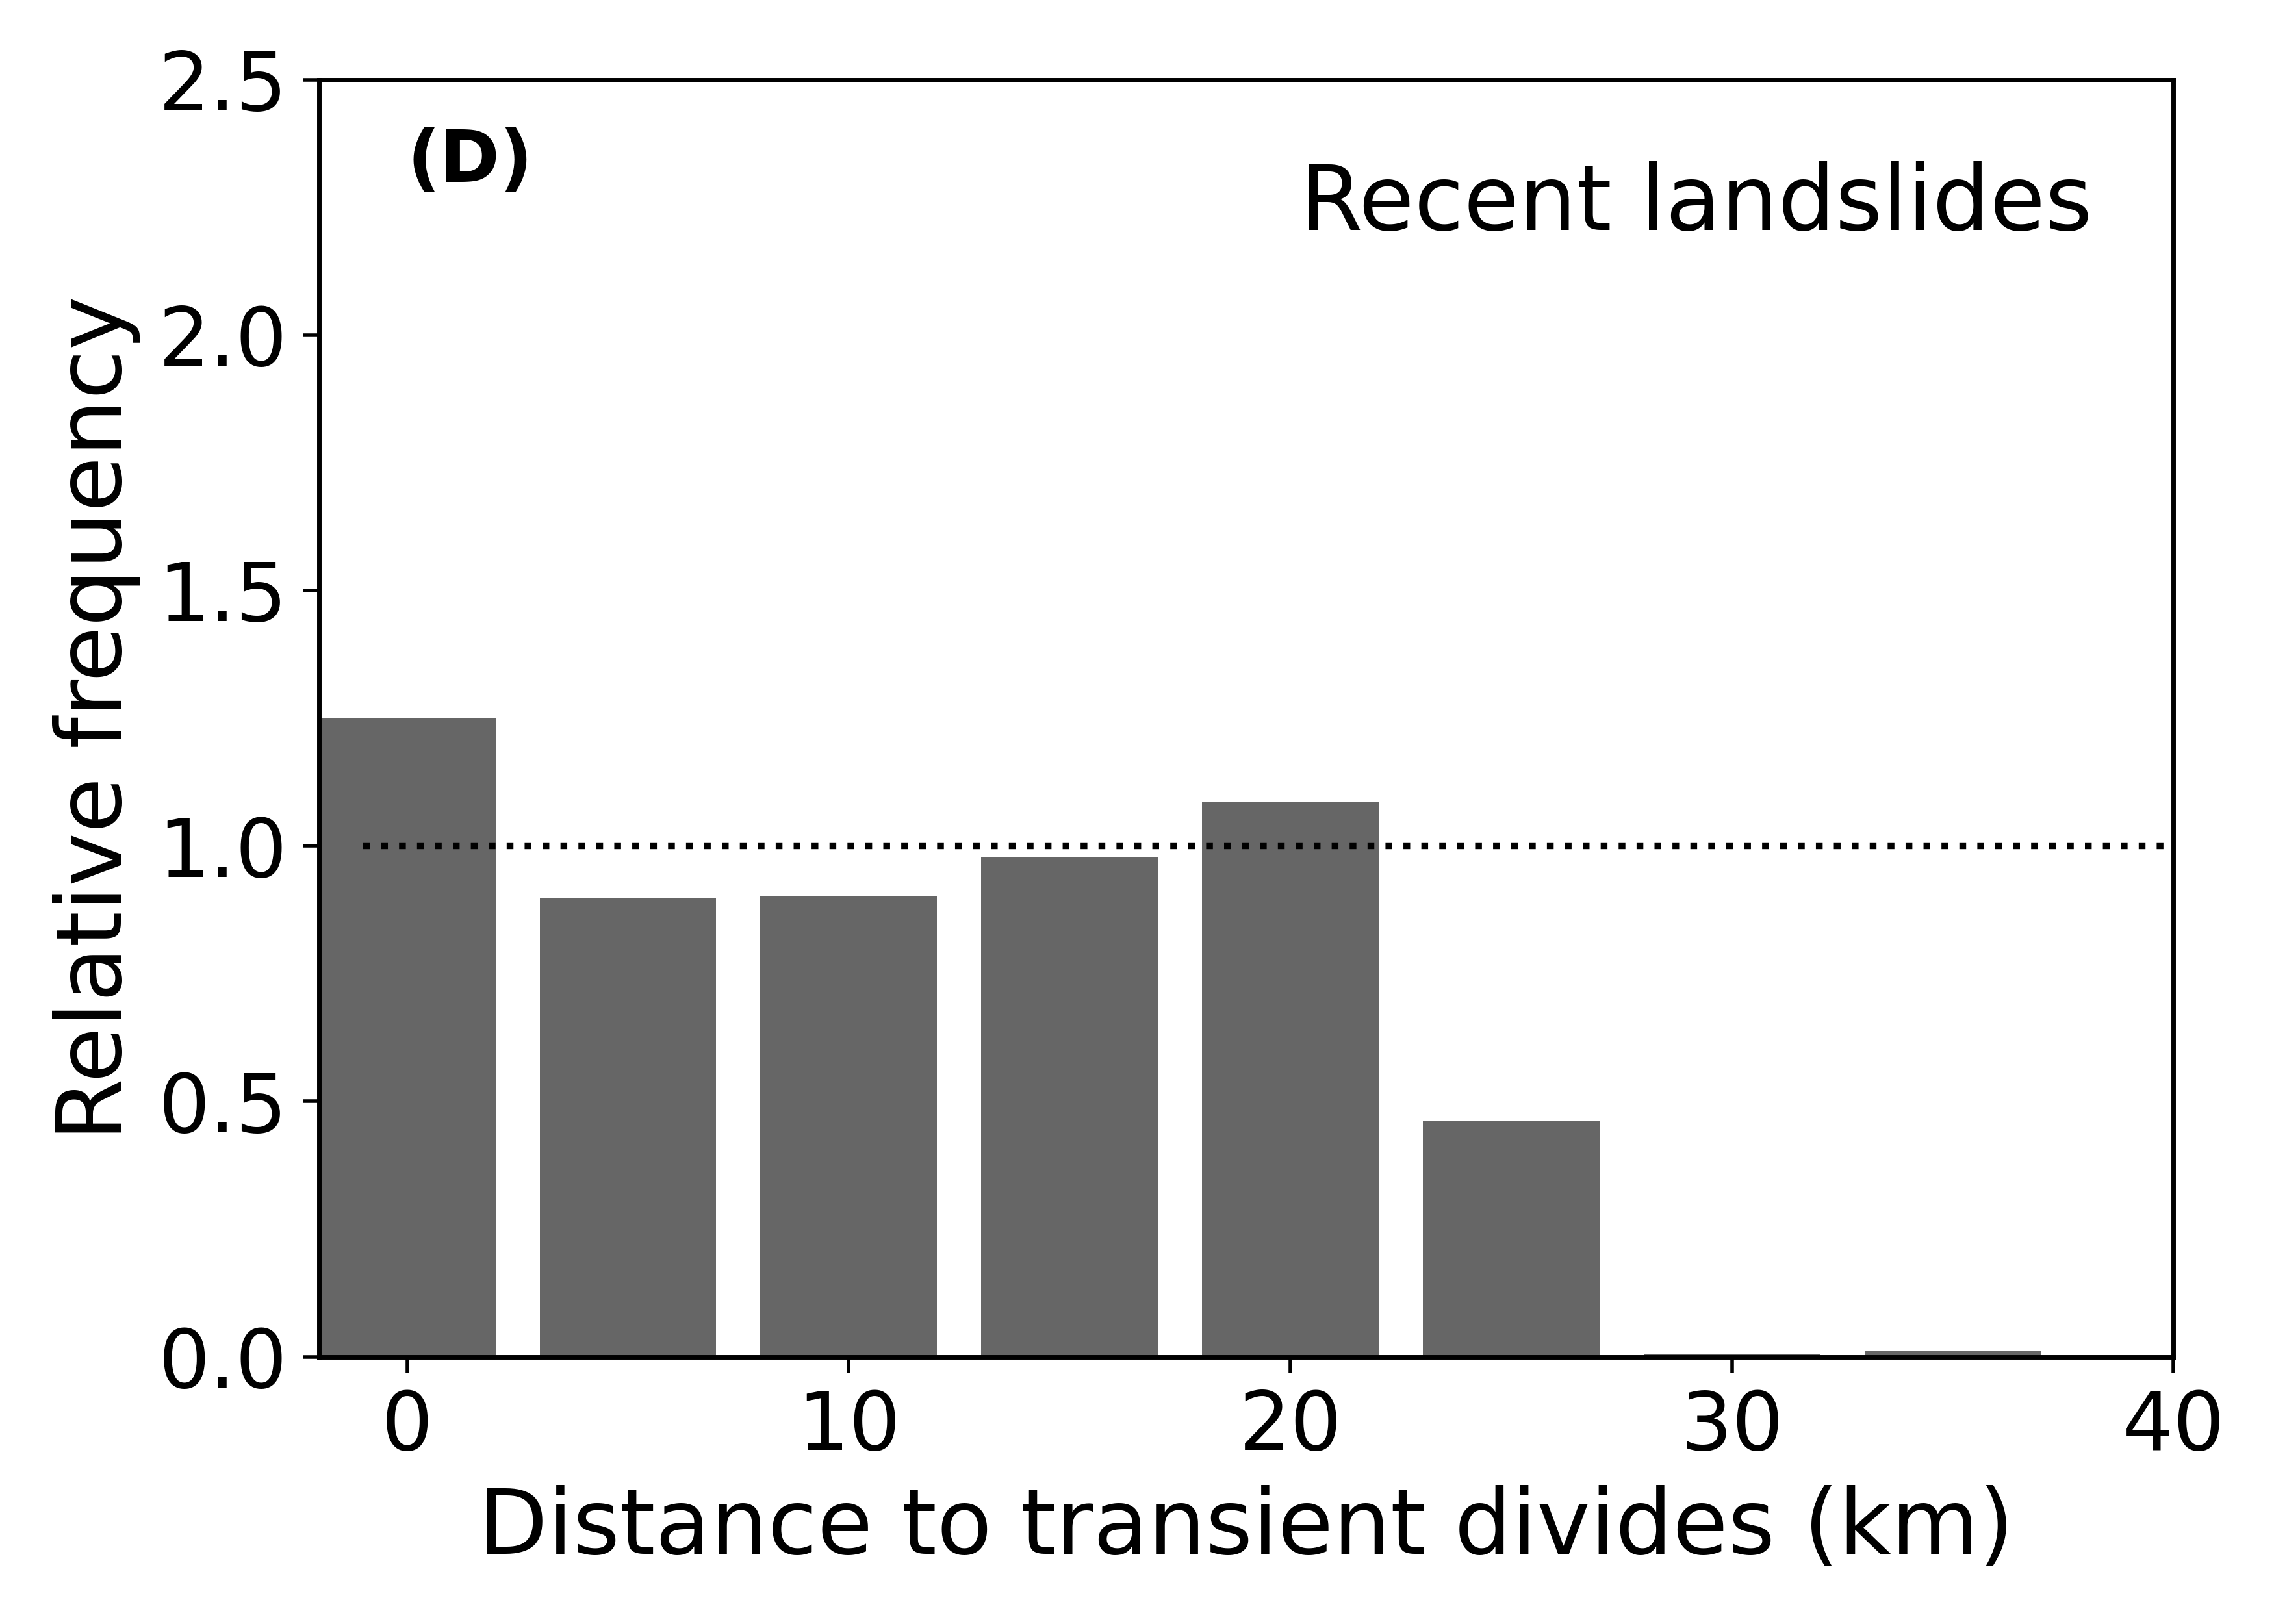
\includegraphics[width=1\textwidth]{Fig10D.png}}
  \end{minipage} 
    \caption{Distribution of $\chi$ along the drainage network of the northern Colombian Andes with prehistoric and recent landslides. Active transient divides are inferred from differing $\chi$ values between main catchments, with divides migrating towards larger $\chi$-values. Red semi-circles} indicate expected direction of catchment capture; T1 to T4 mark dominant divide migrating trends. Histograms show the distance of landslides from the nearest actively migrating drainage divide in 5-km bins, normalized by the fraction of study area at this distance; a relative frequency of 1 marks the expected value for a random distribution.
    \label{fig:rel-rec}
\end{figure}

\end{document}
